\documentclass[11pt,letterpaper,oneside]{phstylee}

\usepackage[mathscr]{eucal}
\usepackage[table]{xcolor}
\usepackage{makeidx}
%\usepackage[ansinew]{inputenc}
%\usepackage[latin1]{inputenc}
\usepackage[final]{pdfpages}
\usepackage[utf8x]{inputenc}
\usepackage[spanish,es-noquoting]{babel}
\usepackage{array}
%\usepackage{epsfig}
%\usepackage{psfig}
%\usepackage{subfigure}
%\usepackage[dvips]{graphicx}
\usepackage{cite}
\usepackage{amsfonts}
\usepackage{amsmath}
\usepackage{amssymb}
\usepackage{amsxtra}
\usepackage{varioref}
\usepackage{multicol}
\usepackage{float}
\usepackage{rotate}
\usepackage{rotating}
\usepackage{color}
\usepackage{enumerate}
\usepackage{pmat}
%\usepackage{theorem}
%\usepackage[pdftex]{graphicx}
\usepackage{graphicx}
%\usepackage{hangcaption}
\usepackage{latexsym}
%\usepackage{stmaryrd}
% \usepackage{euler}
\usepackage{amsthm}
\usepackage{dsfont}
\usepackage{epstopdf}
%\epstopdfsetup{outdir=.}
\DeclareGraphicsExtensions{.pdf,.png,.jpg}
\usepackage{caption}
\usepackage{subcaption}
\usepackage{multirow}
\setcounter{secnumdepth}{5}
\usepackage{algorithm}
\usepackage{algpseudocode}
\usepackage{booktabs}
%\usepackage{fancybox}
%\usepackage{hyperref}
%\usepackage[pdftex,bookmarks,colorlinks]{hyperref} 
%\hypersetup{colorlinks,linkcolor=blue,urlcolor=blue}
%%%%%%%%%%%%%%%%%%%%%
%      DIRECTORIO DONDE BUSCA LAS FIGURAS

\graphicspath{{img/}}
\usepackage{pifont}
\usepackage{textcomp}
\usepackage{subcaption}
\usepackage{pgf}
\usepackage{tikz}
\usepackage{listings}
\usepackage{afterpage}
\usetikzlibrary{shapes,arrows,positioning,calc,shadows}

\addto\captionsspanish{%
\def\bibname{Referencias}%
\def\tablename{Tabla}%
\def\listtablename{ÍNDICE DE TABLAS}%
\def\listfigurename{ÍNDICE DE FIGURAS}
}
\renewcommand{\listfigurename}{ÍNDICE DE FIGURAS}
\renewcommand{\listtablename}{ÍNDICE DE TABLAS}

\newcommand{\comm}[1]{
\noindent\fbox{\parbox{\textwidth}{\begin{center} #1 \end{center}
}}\\}

\usepackage{mdframed}

\newcommand{\midtilde}{\raisebox{0.5ex}{\texttildelow}}

\usepackage{multirow}
\usepackage{etoolbox}
%\patchcmd{\thebibliography}{\section*{\refname}}{}{}{}

\definecolor{colora}{RGB}{102,190,14}
\definecolor{colorb}{RGB}{174,128,3}
\definecolor{colorc}{RGB}{204,51,51}
\definecolor{colord}{RGB}{174,3,128}
\definecolor{colore}{RGB}{120,14,190}
\definecolor{colorf}{RGB}{30,76,201}

%\hyphenation{CONICYT Marco trans-fe-ren-cia pre-li-mi-na-res co-rres-pon-dien-tes de-no-mi-na-dor MIMO res-pec-ti-va-mente}
\renewcommand\thesubsubsection{\Alph{subsubsection}}

\addtolength{\topmargin}{-30pt}

\usepackage[colorlinks=false,linkcolor=black,citecolor=black,hidelinks]{hyperref} %Para evitar recuadros de links.
\linespread{1.1}
\makeindex
\spanishdecimal{.}
\allowdisplaybreaks

%%%%%%%%%%%%%%%%%%%%%%%%%%%%%%%%%%%%%%%%%%%%%%%%%%%%%%%%%%%%
%%%%%%%%%%%%%%%%%%%%%%%%%%%%%%%%%%%%%%%%%%%%%%%%%%%%%%%%%%%%

\begin{document}

\tikzset{
block/.style = {draw, fill=white, rectangle, minimum height=3em, minimum width=3em},
tmp/.style  = {coordinate}, 
sum/.style= {draw, fill=white, circle, node distance=1cm},
input/.style = {coordinate},
output/.style= {coordinate},
pinstyle/.style = {pin edge={to-,thin,black}}
}

%\layout

%--------------------PORTADA--------------------------------

%\setcounter{tocdepth}{2}
%

\pagestyle{empty}


\begin{center}

\large \textbf{UNIVERSIDAD TÉCNICA FEDERICO SANTA MARÍA}

\vspace{3mm}

\normalsize DEPARTAMENTO DE ELECTRÓNICA

\vspace{3mm}

\normalsize VALPARAÍSO-CHILE

\vspace{4mm}
		\begin{figure}[H]
			\centering
			
\includegraphics[width=5.85cm]{usmLogo_1.png}
		\end{figure}
\vspace{2mm}

\Large{\bf SISTEMA DE ADQUISICIÓN DE DATOS PARA DETECTORES DE MUONES}

\vspace{10mm}



\large \textbf{JAIRO ESTEBAN GONZÁLEZ CABEZAS}

\vspace{10mm}

\normalsize
MEMORIA DE TITULACIÓN PARA OPTAR AL TÍTULO DE INGENIERO CIVIL ELECTRÓNICO

\vspace{5mm}

PROFESOR GUÍA

%\vspace{2mm}

DR. GONZALO CARVAJAL
\vspace{5mm}

PROFESOR CO-REFERENTE

%\vspace{2mm}

DR. HAYK HAKOBYAN

\vspace{10mm}

DICIEMBRE, 2020


\end{center}



\cleardoublepage

\vspace{50mm}

\begin{flushright}
  {\emph{\\}}
 \vspace{3mm}
  {\emph{\\}}


 
\end{flushright}
\vspace{170mm}
\begin{flushright}
{\emph{\\}}
\end{flushright}

%
%\newpage
%\thispagestyle{empty}
%\cleardoublepage


%--------------------AGRADECIMIENTOS----------------------

\pagestyle{fancyplain}
\pagenumbering{roman}
\cleardoublepage
\newpage


%\chapter*{Agradecimientos}
%%Agradecimientos

agradecer
%\afterpage{\thispagestyle{empty}\null\newpage}


%--------------------RESUMEN----------------------

%\chapter*{Resumen}
%Los muones son partículas subatómicas originadas por la interacción y decaimiento de otras partículas elementales. Los muones se originan principalmente por radiación cósmica proveniente del espacio exterior y son capaces de penetrar en la atmósfera, incluso llegando a la corteza terrestre y atravesando la materia que encuentran a su paso. Medir la energía de un muón luego de su paso a través de la materia permite conocer la densidad de los materiales atravesados, por lo que la detección de muones es un área de estudio interesante para análisis de terrenos y estructuras.

El ``Sistema de adquisición de datos para detectores de muones'' nace como un requerimiento del CCTVal (Centro Científico Tecnológico de Valparaíso) en  el marco del proyecto ``sTGC Minería'', cuyo objetivo es realizar tomografías muónicas de terreno minero mediante detectores sTGC. Un detector emite señales eléctricas que representan la posición y la energía asociadas al paso de un muon, por lo que se requiere un sistema de adquisición que capture estas señales y las entregue a un posterior sistema de análisis para la caracterización del muon detectado.

En esta memoria de titulación se desarrolla un sistema de adquisición prototipo que cumple las funciones de muestrear señales digitales provenientes de un detector, discriminar la autenticidad de la detección mediante la lectura de una señal externa de disparo, y enviar la información capturada hacia un computador externo con el fin de almacenar y procesar los datos adquiridos. El sistema de adquisición debe ser capaz de muestrear 16 señales digitales cuyos tiempos de duración están en el orden de los nanosegundos, y debe diseñarse pensando en su replicación y escalamiento para facilitar la conexión de detectores adicionales. El trabajo de diseñar este sistema sienta un precedente importante para CCTVal, por lo que el proceso de desarrollo y los conocimientos adquiridos se documentan conjuntamente en esta memoria y en el repositorio de Git asociado.

\textbf{Palabras claves:} Detectores sTGC,  Muones, FPGA, Adquisición de Datos.
%
%\newpage
%\thispagestyle{empty}
%\cleardoublepage
%
%\chapter*{Abstract}
%%abstract

abstract

\textbf {Keywords:} words, words.
%
%\newpage
%\thispagestyle{empty}
%\cleardoublepage
%
%%--------------------ÍNDICE---------------------------------
%\listoffigures
%
%\newpage
%\thispagestyle{empty}
%\cleardoublepage
%
%\listoftables
%
%\newpage
%\thispagestyle{empty}
%\cleardoublepage
%
%\tableofcontents
%
%\newpage
%\thispagestyle{empty}
%\cleardoublepage

%%-------------------CAPÍTULOS-------------------------------
%
%%%%%%%%%%%%%%%%%%%%%%%%%%%%%%%%%%%%%%%%%%%%%%%%%%%%%%%%%%%%%

\pagenumbering{arabic}

%\chapter{Introducción}
%\label{cap:introduccion}
%%Introducción


\section{Contextualización}
	\par El proyecto ``Sistema de adquisición de datos para detectores de muones'' nace como un requerimiento del Centro Científico Tecnológico de Valparaíso (CCTVal) para aplicaciones de física de partículas, en el marco del proyecto ``sTGC Minería''. 
	
	\par Uno de los objetivos principales de ``sTGC Minería'' es realizar tomografías muónicas de terreno minero mediante detectores de partículas provenientes de radiación cósmica, idea similar a la que se utiliza para encontrar criptas y cavernas en pirámides egipcias. La detección de estos muones implica una serie de etapas y detectores desarrollados con tecnologías que se utilizan en experimentos tales como ATLAS, en CERN. Particularmente en ``sTGC Minería'', se requiere un sistema que sea capaz de captar las señales generadas por los detectores y que determine de manera fiable y precisa aquellas zonas del detector por las cuales ha pasado un muón.
	
	\par El proyecto ``Sistema de adquisición de datos para detectores de muones'' cumplirá con las funciones de adquirir, discriminar y procesar la información captada desde el detector, para así contribuir a la tomografía muónica del terreno.

\section{Objetivos del proyecto}\label{sec:objetivos}
	\par El presente proyecto tiene como objetivo principal detectar la posición del paso de muones en un detector de configuración matricial, indicando el o los cuadrantes que han sido excitados por el paso de las partículas de manera fiable y eficiente, logrando captar gran cantidad de señales de manera íntegra en el tiempo apropiado para ello.
	\par Es requisito del proyecto que este sistema sea concebido como una herramienta adaptada para operar con detectores de mayor tamaño o con arreglos de detectores individuales, permitiendo el análisis de zonas de mayor área o el estudio de trayectorias de partículas con detectores superpuestos. Esto implica que el sistema debe ser de naturaleza modular y expandible, sobre todo en la cantidad de señales que es capaz de procesar.
	\par Como objetivos secundarios, se espera que este proyecto sea una herramienta replicable y esté disponible para ser utilizado en nuevos proyectos y experimentos del centro de investigación. Se espera también que sea un aporte al conocimiento sobre la implementación de sistemas electrónicos para la detección y análisis de partículas utilizando estas tecnologías, ya que será uno de los primeros en ser desarrollados y probados por el centro.\\								


%	\begin{figure}[H]
%		\centering
%		
%		\tikzstyle{externo} = [rectangle, rounded corners, minimum width=2cm, minimum height=1cm,text centered, draw=black, fill=blue!30]
%		\tikzstyle{fpga} = [rectangle, rounded corners, minimum width=3cm, minimum height=2.5cm,text centered, draw=black, fill=green!30]
%		\tikzstyle{flecha} = [thick,->,>=stealth]   
%		
%		\begin{tikzpicture}[node distance=1.5cm, thick,scale=0.9, every node/.style={scale=0.9\\}]
%			
%			\node (disparo) [externo] {Disparo};
%			\node (detector) [externo, below of=disparo] {Detector};
%			\node (asd) [externo, right of=detector, xshift=1cm] {ASD};
%			\node (disc) [fpga, right of=detector, xshift=2.5cm, yshift=-0.5cm, anchor=south west] {Discriminador};
%			\node (pros) [fpga, right of=disc, xshift=2cm] {Procesamiento};
%			\node (res) [fpga, right of=pros, xshift=2cm] {Análisis};
%			
%			\draw [flecha] (disparo) --  (disc.west |- disparo);
%			\draw [flecha] (detector) -- (asd);
%			\draw [flecha] (asd) -- (disc.west |- asd);
%			\draw [flecha] (disc) -- (pros);
%			\draw [flecha] (pros) -- (res);
%			
%		\end{tikzpicture}
%		
%		\caption{Diagrama de bloques del sistema. En azul se presentan las etapas previas al proyecto que ya se encuentran desarrolladas y sobre las cuales no se tiene control. En verde se ilustran las etapas pendientes y que pueden ser desarrolladas en este proyecto. El disparo corresponde a la señal digital que indica si la partícula detectada es un muón y el ASD es un acondicionador de señal que genera pulsos digitales a partir de los pulsos analógicos captados.}
%		\label{fig:diagrama}
%	\end{figure}

\section{Trabajo a Desarrollar}

	\par Como primeras labores, será necesario aprender sobre la tecnología y el funcionamiento del detector para así asegurar que los datos están siendo tratados de manera adecuada. Esto implica conocer su resolución, la naturaleza de las señales y las restricciones de tiempo propias del sistema. 
	
	\par Posteriormente, se procederá a investigar sobre técnicas para la captación y procesamiento de estas señales, definiendo así las alternativas disponibles para realizar el proyecto. Es sabido que las tomografías por rayos cósmicos son tecnología existente, y se cuenta también con la existencia de aplicaciones que se han desarrollado en laboratorios de física de partículas europeos, como el CERN. Estas últimas tienen como preferencia la utilización de FPGA para el desarrollo de este tipo de sistemas.
	
	\par Una vez que se tengan claras la herramientas y requisitos, se definirá y planificará en detalle la solución a implementar de acuerdo a los objetivos del proyecto. Se estima que la implementación se llevará a cabo en una FPGA, lo que implicará definir los módulos que compondrán cada etapa del sistema antes de implementarlo como tal. En principio. estas etapas corresponderán a las de discriminación, procesamiento y análisis, como se ilustra en la figura \ref{fig:diagrama}. 
	
	\par Finalmente, se realizarán pruebas de manera incremental con cada una de las etapas a desarrollar. Estas pruebas se podrán realizar con partículas intencionalmente dirigidas hacia la superficie del detector y posteriormente con rayos cósmicos, para así comprobar y observar el correcto funcionamiento del sistema.

\section{Evaluaciones a Realizar}
	
	\par En primera instancia, se evaluará la capacidad del sistema de adquirir señales provenientes del detector, con apoyo de partículas dirigidas a él mediante fuentes radioactivas. Luego, se podrá probar que las señales detectadas correspondan solo a muones, utilizando como referencia la señal de disparo existente para dicho fin, comprobando que no hayan falsos positivos y que no se pierdan señales que debieron ser consideradas por el sistema. Una vez que se tenga certeza del funcionamiento de la adquisición y discriminación de señales, se probará que el sistema sea capaz de identificar la posición de partículas por cuadrantes específicos del detector, también con apoyo de fuentes radioactivas. Finalmente, se pondrá a prueba la capacidad del sistema para entregar información completa sobre el paso de partículas en la superficie del detector.
	
	

\section{Resultados Esperados}
	\par Se espera que este sistema sea capaz de generar información suficiente para representar la ubicación del paso de las partículas en la superficie del detector según la resolución de este.
	\par El sistema deberá ser capaz de captar cantidades pares arbitrarias de canales, discriminando partículas mediante la utilización de las señales de disparo disponibles.
	\par La información generada pasará a etapas siguientes de análisis detallado o de representación gráfica, por lo que se espera que el sistema sea capaz de entregar información pertinentemente ordenada, procesada y seleccionada para dichos fines.\\
	 
%La presente tesis se ordena como sigue: El capítulo \ref{cap:introduccion} presenta la introducción al tema,....




%
%\newpage
%\thispagestyle{empty}
%\cleardoublepage
%
%\chapter{Estado del arte}
%\label{cap:art}
%%Estado del arte y arquitectura propuesta
\section{Estado del Arte}
	\par En física de alta energía, los detectores de partículas cumplen un rol fundamental. A través de ellos se puede observar y medir la naturaleza de diferentes partículas fundamentales. Para que esto sea posible, es necesario implementar sistemas de adquisición de datos (DAQ, por su sigla en inglés), capaces de tomar la información captada por los detectores, haciéndola procesable y comprensible.
	\par El sistema a desarrollar en este proyecto de titulación está pensado para acompañar a detectores de muones provenientes de rayos cósmicos, basados en tecnología desarrollada en CERN para el estudio de física de partículas. Este sistema será el encargado de filtrar las señales emitidas por el detector y entregar información sobre el paso de muones en él.
	\par Previo al desarrollo y diseño de este sistema, es pertinente conocer el estado del arte de sistemas de adquisición de datos para física de partículas, especialmente los utilizados en CERN, para así contrastar y rescatar las diferentes estrategias y tecnologías empleadas actualmente en esta área del conocimiento.
	\par En las siguientes páginas se mencionan distintos sistemas relacionados a esta temática, destacando ideas sobre el esquema general de adquisición de datos, tecnologías que se utilizan actualmente para construirlos y  métodos para adquirir y procesar las señales captadas.
	
	\section{Estructura esencial y arquitectura propuesta}
	\par ¿Cuáles son las etapas esenciales que un DAQ debe poseer? En esencia se requiere de una primera etapa de interfaz de lectura directamente de los detectores (Readout), las cuales suelen poseer amplificadores, modeladores de pulsos, memorias y digitalizadores. Una segunda etapa suele consistir en el preprocesamiento de las señales, extrayendo la información básica y formando estructuras de datos pertinentes. Finalmente, está la etapa de procesamiento fuera del detector, donde se realiza el análisis e interpretación de los datos.
	
	\par En este proyecto de titulación, la primera etapa la lleva a cabo la tarjeta acondicionadora ASD (Amplifier Shaper Discriminator), diseñada para detectores del proyecto ATLAS. Las etapas restantes serán diseñadas pensando en la aplicación específica de este proyecto.

\newpage
\section{Sistemas para la Adquisición de Datos en Física de Partículas}

\subsection{LabPet II}

\par Como referencia para el diseño del sistema de adquisición, se han investigado detectores como los descritos en \cite{Basiladze2017Methods1} y \cite{Basiladze2017Methods2}, enfocados a detección de partículas en diferentes rubros y condiciones.
\par Dentro de la variedad de detectores estudiados, el LabPet II de Larissa Njejimana \cite{Njejimana2013DesignImaging} presenta una estructura clara e interesante. Este detector posee un DAQ distribuido en tres FPGAs, contando con etapas para recolectar, procesar y transmitir la información obtenida. Una primera etapa cosiste en registrar el tiempo, la energía y la posición de las partículas sensadas; una segunda etapa ordena cronológicamente los eventos capturados y una tercera etapa que agrupa eventos coincidentes, calculando además la tasa de eventos aleatorios ocurridos. La figura \ref{fig:njejimana} ilustra este sistema.

\par Si bien dicho detector está diseñado para otro tipo de partículas (positrones), la naturaleza de las señales es muy similar, y por lo tanto la lógica para su adquisición y procesamiento es comparable. Aún así, la cantidad de señales que es capaz de manejar dicho dispositivo ronda las 64 señales por módulo, a tasas cercanas a los 2 millones de eventos por segundo, las que comparativamente sobrepasarían las necesidades del sistema a desarrollar en este proyecto de titulación. Por ejemplo, los rayos cósmicos cruzan el planeta tierra a aproximadamente 1 rayo cósmico por minuto en un área de un centímetro cuadrado, muy por debajo de lo que se espera en el LabPET II.

\par Del sistema de adquisición para el detector anteriormente mencionado, se destaca la utilización de multiplexores, serializadores/deserializadores y memorias de almacenamiento temporal (buffer). Dada la naturaleza y cantidad de eventos, se hace necesario serializar la información, ya que de otro modo sería necesario construir dispositivos con muchos puertos de entrada o incluir varios del mismo tipo. Además, debido a la frecuencia de aparición de eventos, se hace obligatoria la existencia de buffers para el almacenamiento de la información, para así procesarlos y transmitirlos a etapas siguientes a tasas menores. Es destacable también la utilización de métodos para ordenar cronológicamente los eventosy la utilización del método TOT (Time-over-threshold) para el calculo de energía y datos temporales de pulsos analógicos. 


\begin{figure}[H]
	\centering
	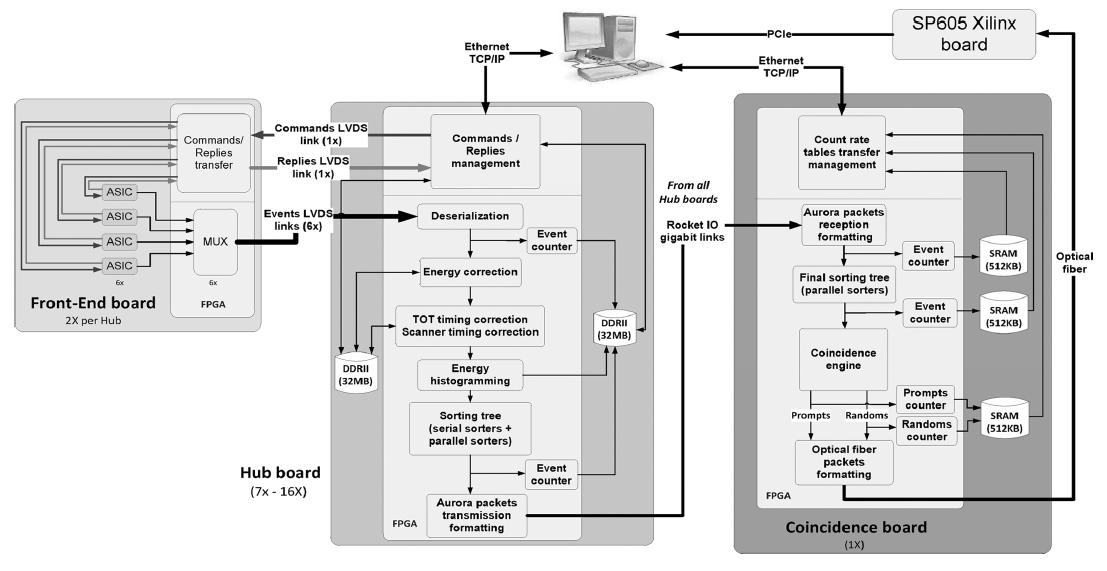
\includegraphics[scale=0.55]{imagenes/njejimana.png}
	\caption{Diagrama de bloques del sistema de adquisición de datos para LabPET II \cite{Njejimana2013DesignImaging}}
	\label{fig:njejimana}
\end{figure}

\newpage
\subsection{PET 4D}

\par Otro sistema de referencia es el DAQ para un detector PET 4D \cite{Marcatili2011DevelopmentDetector}, similar al LabPET II. Este dispositivo permite capturar gran cantidad de señales provenientes de arreglos matriciales de fotomultiplicadores. Se caracteriza principalmente por poseer una tarjeta madre central en la cual es posible conectar hasta 18 tarjetas de adquisición. Cada una de estas últimas cuenta con 8 o hasta 32 canales para la adquisición de pulsos provenientes del detector, encargándose de capturar, procesar y enviar información a la placa madre.
Las señales son capturadas por ASICs (Application Specific Integrated Circuits), muestreadas por conversores análogo-digitales, procesadas por una FPGA y controladas por otra FPGA (etiquetada como la placa madre). El procesamiento se encarga de calcular energía y datos temporales, mientras que el control final relaciona los eventos que hayan sido temporalmente coincidentes y calcula el tiempo de vuelvo de las partículas con apoyo de un conversor de tiempo a digital (TDC).

\par Este sistema destaca por su modularidad, la cual permite escalamiento. En contraste con LabPET II, se sustituye la serialización de datos con la presencia de varias placas adquisidoras de datos, preprocesando la información antes de llegar a la FPGA principal. Cabe destacar que esta arquitectura está relacionada con la necesidad de encontrar múltiples eventos simultáneos en distintas ubicaciones físicas, requerimiento que no está presente en el sistema que se planea diseñar para este proyecto de titulación. La figura \ref{fig:marcatili} ilustra la arquitectura de este sistema.

\begin{figure}[H]
	\centering
	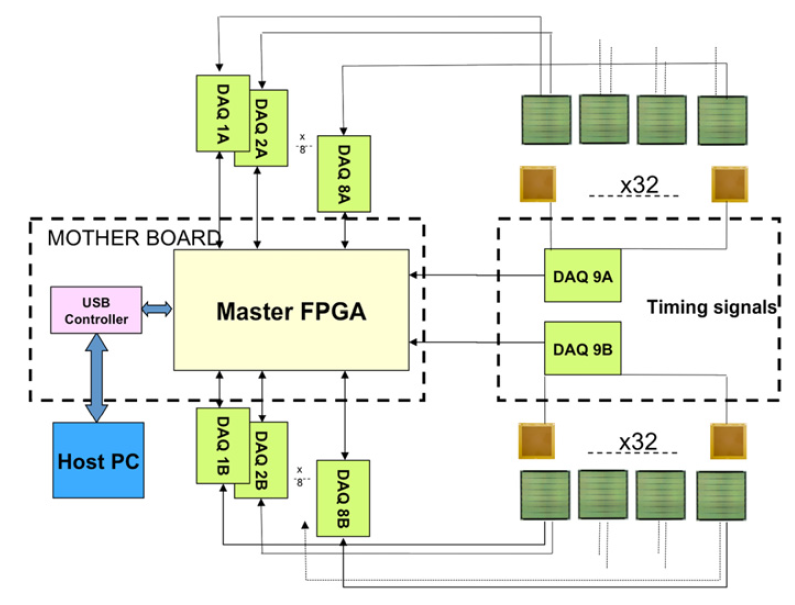
\includegraphics[scale=0.4]{imagenes/marcatili.png}
	\caption{Diagrama de bloques del sistema de adquisición de datos para Detector PET 4D \cite{Marcatili2011DevelopmentDetector}}
	\label{fig:marcatili}
\end{figure}

\newpage
\subsection{ATLAS}

\par Finalmente, la referencia más importante corresponde a la del experimento ATLAS, donde se utiliza la misma tecnología de detectores y la misma interfaz de adquisición (ASD) en una de sus etapas, como se mencionada en \cite{Spieler2012ElectronicsAcquisition}.

\par Este experimento intercepta grupos de partículas provenientes de haces de protones acelerados en el Gran Colisionador de Hadrones (LHC) en CERN. Estos grupos de partículas producen colisiones espaciadas en el tiempo en aproximadamente $25\mu s$ entre si, cada una produciendo cerca de 23 interacciones con el detector, que junto a otros factores implica cerca de $10^9$ eventos cada segundo \cite{Whiteson2016TheSystem}. La magnitud, tasa de aparición y nivel de energía de estos eventos son las principales razones de la complejidad tecnológica de este detector.

\par Este detector posee dos etapas previas de selección de eventos, donde la primera etapa involucra detectores de muones y calorímetros, mientras que la segunda involucra algoritmos distribuidos en varios computadores. La figura \ref{fig:spieler} ilustra la interfaz para la captura de los pulsos generados por muones en los detectores (TGC).


\begin{figure}[H]
	\centering
	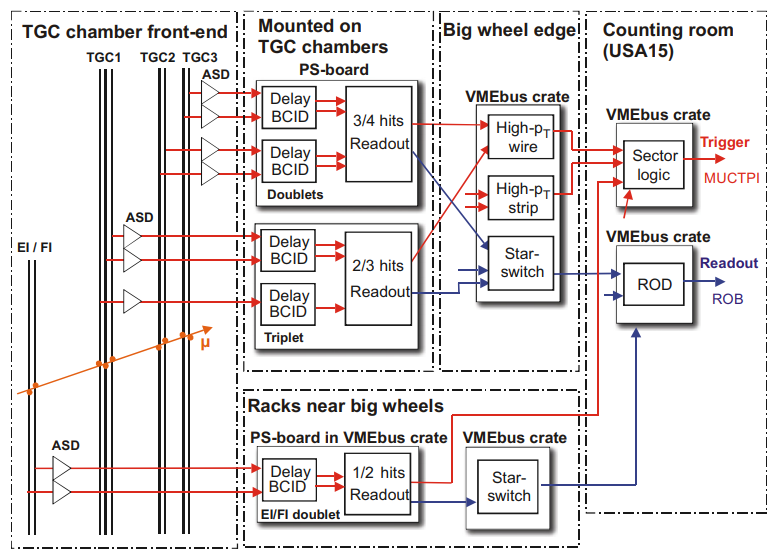
\includegraphics[scale=0.6]{imagenes/spieler.png}
	\caption{Diagrama de la interfaz de lectura para detectores de muones \cite{Spieler2012ElectronicsAcquisition}. Los muones se representan con el símbolo $\mu$. Existen 3 capas de detectores, por lo tanto se observan 3 bloques que incluyen retardos, selección y captura de los pulsos. La información capturada formará parte de la señal de disparo del primer nivel (Lever 1 Trigger).}
	\label{fig:spieler}
\end{figure}

\par Luego de generarse la primera señal de disparo, se da paso a la adquisición de datos en la tarjeta de lectura del detector (Readout System), enviando paralelamente información sobre regiones de interés a analizar, con el fin de llevar a cabo la segunda etapa de selección de eventos mediante el disparo de alto nivel (High-Level Trigger). Esta segunda señal de disparo utiliza software distribuido en cerca de 2000 computadores conectados a una red Ethernet y filtra eventos en función a muestras de datos pertenecientes a las regiones de interés calculadas por la etapa de disparo anterior, como se describe en \cite{Colombo2015Data-flowCase}. Finalmente, los eventos seleccionados son trasferidos y  almacenados en los bancos de datos del centro de investigación. La figura \ref{fig:colombo} ilustra las etapas mencionadas.

\begin{figure}[H]
	\centering
	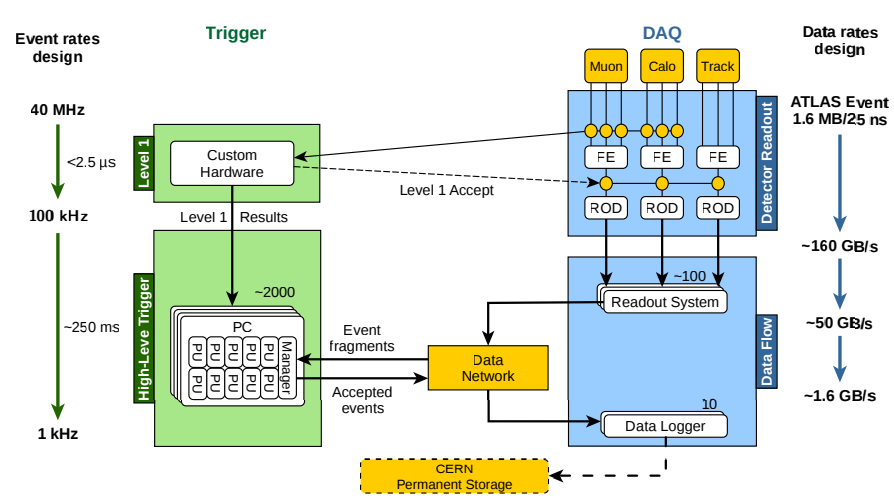
\includegraphics[scale=0.7]{imagenes/colombo.png}
	\caption{Diagrama del sistema de disparo y adquisición de datos en el experimento ATLAS. \cite{Colombo2015Data-flowCase}}
	\label{fig:colombo}
\end{figure}

\par Entrando en detalle, según se indica en \cite{Whiteson2016TheSystem}, el verdadero sistema de adquisición de datos para este experimento es el software distribuido en red, capaz de discriminar, procesar y transferir los eventos seleccionados a los bancos de datos. El sistema lectura (Readout System) en conjunto con el disparo de primer nivel solo serían un equivalente a una interfaz de captura muy sofisticada, más que las observadas en otros detectores, pero para el caso de este proyecto de titulación es comparable al sistema de adquisición que se desea diseñar.

\par El sistema de lectura consiste en una tarjeta llamada ROBIN, compuesta de buffers, chips de comunicación, memoria flash, procesador y una FPGA, como se ilustra en la figura \ref{fig:whiteson}

\begin{figure}[H]
	\centering
	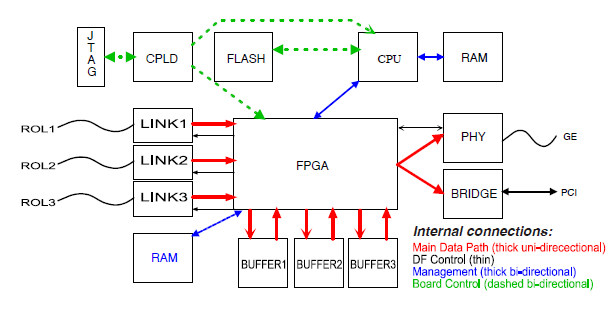
\includegraphics[scale=0.7]{imagenes/whiteson.png}
	\caption{Diagrama de la tarjeta de lectura ROBIN en ATLAS \cite{Whiteson2016TheSystem}.}
	\label{fig:whiteson}
\end{figure}

\newpage
\par La lógica descrita al interior de dicha FPGA se ilustra en la figura \ref{fig:whiteson2}. Se observa que su labor es principalmente controlar los buffers de datos, traspasar los eventos captados hacia la siguiente etapa y eliminar los datos descartados por la señal de disparo de alto nivel.

\begin{figure}[H]
	\centering
	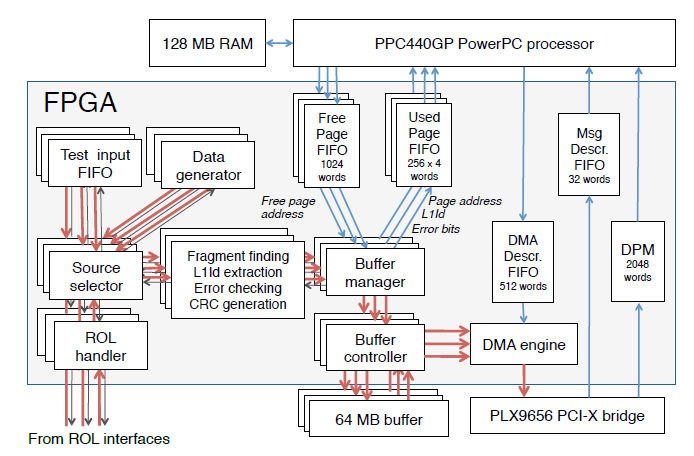
\includegraphics[scale=0.7]{imagenes/whiteson2.png}
	\caption{Diagrama de bloques de la FPGA en ROBIN \cite{Whiteson2016TheSystem}.}
	\label{fig:whiteson2}
\end{figure}

\par Si bien este detector es comparativamente más complejo que los anteriores, presenta elementos comunes es su composición, sobretodo en la utilización de ASICs y FPGA para captura y control de los datos adquiridos. Se asemeja funcionalmente al PET 4D, en el sentido de implementar múltiples instancias de hardware equivalente, para así lograr manejar mayores cantidades de datos, brindando también mayor control e independencia en cada uno de ellos. El fuerte de este detector radica en su conectividad en red y sistemas distribuidos, necesarios para la gran cantidad de datos simultáneos que deben ser procesados. 

\newpage
\section{Conclusiones}
\par Habiendo comparado y estudiado diferentes estilos de detectores y sistemas de adquisición, es claro que la tendencia es la utilización de ASICs en etapas de primera lectura y de FPGAs en etapas de manejo de datos y preprocesamiento, principalmente debido a la magnitud temporal de las señales, a la alta necesidad de precisión en su sincronización, y a la gran cantidad de señales de entrada que deben ser atendidas.

\par Los elementos más utilizados y recomendados a implementar son los buffers de almacenamiento, principalmente para ajustar la tasa de transmisión de datos de la captura hacia las siguientes etapas de procesamiento, que suelen ser más lentas. En el sistema que se planea diseñar esto no sería un problema, ya que la tasa de eventos es muy baja en comparación a los detectores estudiados. Aún así, pueden ser útiles para el escalamiento de los detectores.

\par El concepto de serialización de datos estuvo principalmente presente en el detector LabPET II. Es pertinente considerarlo, sobretodo para el escalamiento del detector de muones. En caso de requerir cubrir un área mayor o con varias capas superpuestas de detectores, será necesario captar mayor cantidad de señales. Es allí donde se debe decidir si es recomendable comenzar con serialización de datos o con paralelismo de hardware. Además, dado que es necesario tener noción del tiempo de ocurrencia de los eventos, podría asociarse este dato a cada pulso, facilitando la implementación de serialización de datos. Esto no sería una desventaja, ya que no existe real necesidad de procesar datos de manera rápida y simultanea, reduciendo costos en hardware, pero aumentando esfuerzos de ingeniería.

\par Para el caso de preprocesamiento, selección, formateo y transmisión de datos puede se considerar agregar procesadores dedicados en conjunto con la FPGA principal, que si bien no fueron encontrados textualmente en los ejemplos indicados, sí pueden ser de utilidad, sobretodo dada la existencias de chips que incluyen FPGA en conjunto con procesadores, como los SoC (System on Chip) Zynq.

\par Finalmente, puede ser interesante incluir métodos de TDC para conversión de la señal digital generada por la placa acondicionadora ASD. La duración de esta señal tiene relación con la amplitud y la energía de los pulsos analógicos captados, lo que podría ser muestreado con una implementación similar a la indicada en \cite{Arpin2010AResources}.


\section{Arquitectura propuesta para el proyecto}\label{sec:arqui_propuesta}
\subsection{Disposición del detector}\label{sec:orga_detector}

%
%\newpage
%\thispagestyle{empty}
%\cleardoublepage
%
%\chapter{Alternativas de Solución}
%\label{cap:alternatives}
%\par En el documento Estado del Arte para Proyecto de Titulación \cite{Gonzalez2020EstadoTitulacion} se compararon tres sistemas diferentes para la implementación de adquisición de datos para física de partículas. En ellos destacan aspectos comunes de implementación: etapas de detección de eventos, memorias para almacenamiento temporal, procesamiento de los datos y la utilización de FPGA como herramienta principal para la implementación del hardware.

\par En el presente documento se detallan diferentes opciones basadas en los ejemplos mencionados y en los requerimientos del proyecto, con el objetivo de comparar sus características y escoger la alternativa más adecuada. Se compararan aquí aspectos como el costo, simplicidad, desempeño y disponibilidad de las herramientas y equipos necesarios para su implementación.

\par Se incluyen también los requisitos mínimos que deben cumplir las alternativas propuestas y el esquema básico que el proyecto tiene como objetivo para su funcionamiento.

\begin{figure}[H]
    \centering
    
    \tikzstyle{externo} = [rectangle, rounded corners, minimum width=2cm, minimum height=1cm,text centered, draw=black, fill=blue!30]
    \tikzstyle{fpga} = [rectangle, rounded corners, minimum width=3cm, minimum height=2.5cm,text centered, draw=black, fill=green!30]
    \tikzstyle{flecha} = [thick,->,>=stealth]   
    
    \begin{tikzpicture}[node distance=1.5cm]

        \node (disparo) [externo] {Disparo};
        \node (detector) [externo, below of=disparo] {Detector};
        \node (asd) [externo, right of=detector, xshift=1cm] {ASD};
        \node (disc) [fpga, right of=detector, xshift=2.5cm, yshift=-0.5cm, anchor=south west] {Discriminador};
        \node (pros) [fpga, right of=disc, xshift=2cm] {Procesamiento};
        \node (res) [fpga, right of=pros, xshift=2cm] {Análisis};
        
        \draw [flecha] (disparo) --  (disc.west |- disparo);
        \draw [flecha] (detector) -- (asd);
        \draw [flecha] (asd) -- (disc.west |- asd);
        \draw [flecha] (disc) -- (pros);
        \draw [flecha] (pros) -- (res);

    \end{tikzpicture}

    \caption{Diagrama de bloques del sistema. En azul se presentan las etapas previas al proyecto que ya se encuentran desarrolladas y sobre las cuales no se tiene control. En verde se ilustran las etapas pendientes y que pueden ser desarrolladas en este proyecto. El disparo corresponde a la señal digital que indica si la partícula detectada es un muón y el ASD es un acondicionador de señal que genera pulsos digitales a partir de los pulsos analógicos captados.}
    \label{fig:diagrama}
\end{figure}

\section{Alternativas de Solución}
\subsection*{Esquema General}
\par Tal como se ha planteado en informes anteriores, el esquema básico a implementar es el indicado en la figura \ref{fig:diagrama}. Se requieren al menos tres etapas esenciales: discriminar, procesar y analizar. Discriminar se refiere a distinguir entre aquellos eventos que corresponden un muón de aquellos que no, descartando estos últimos. Procesar implica utilizar los pulsos escogidos, formar una estructura que los relacione como un solo evento y posiblemente incluir información de ellos, como una marca temporal y la duración de los pulsos captados en dicho evento. 
\par La etapa de análisis implica mayor complejidad y puede extenderse para abarcar distintos niveles. El análisis más básico implica leer un evento e inferir la región del detector que fue excitada por el paso del muón. Niveles siguientes implicarían estimar la energía del muón, incluir mayor precisión espacial, correlacionar con eventos anteriores o incluso trazar la trayectoria  del paso de la partícula al superponer los datos de eventos originados en otros detectores.

\newpage
\subsection*{Requisitos}
\par Las alternativas aquí propuestas deberán cumplir con las especificaciones mínimas necesarias para captar los pulsos digitales provenientes del detector de muones. Estos requisitos son los siguientes:

\begin{itemize}
    \item Se debe contar con al menos 32 pares de entradas bajo el estándar LVDS, con el fin de conectar al menos 2 tarjetas ASD (Amplificator Shaper Discriminator) utilizadas cada una como la interfaz de detectores de 16 canales.
    \item Es importante contar con un reloj presente o sintetizable de una frecuencia mayor a 100[MHz], lo más cercano a 1[GHz] posible, con el fin de captar la duración de los pulsos y el momento de aparición de un evento con la mayor precisión disponible.
    \item Se debe considerar que la señal de disparo que entrará al sistema estará desfasada cerca de 100[ns] respecto al paso real de los muones por el detector, siendo necesaria la implementación de delays para las señales capturadas o un sistema capaz de distinguir la ocurrencia de eventos y disparos en el tiempo.
    \item  Se debe tener la capacidad de mantener señales sincronizadas, guardar información en memorias temporales y llevar cuenta del transcurso del tiempo entre eventos.
    \item Es requisito que la implementación de la alternativa permita escalamiento para agregar nuevos detectores adyacentes con el fin de aumentar el área de prueba, así como también sincronizarse con detectores paralelos para trazar trayectorias de las partículas captadas.
\end{itemize}

\par En cuanto a los requisitos de tiempo y reloj de operación anteriormente indicados, estos se deben esencialmente a que la duración de un pulso digital proveniente de un detector podría estar entre 1[ns] y 40[ns]\cite{1999ATLASICs}. Este ancho de pulso tiene correlación con la amplitud del pulso análogo original y el error en su medición implicará menor precisión en la estimación de esta variable.

\par Respecto a la tasa de aparición de pulsos consecutivos, es poco probable que ocurran eventos simultáneos o cercanos. Se espera que la tasa de muones por centímetro cuadrado sea de un muón por minuto, lo que en los $15[cm^2]$ representados por una señal de detector implicaría cerca de 15 muones por minuto o $2,5*10^{10}$ muones cada 100 [ns], lo que se traduce a una muy baja probabilidad de eventos simultáneos o incluso cercanos. De hecho, la tasa de detección de muones puede disminuir estando bajo tierra y se planea que la toma de una muongrafía conlleve un tiempo prolongado de exposición a rayos cósmicos. Esto conduce a la conclusión de que ignorar posibles eventos simultáneos o adyacentes no tendrá implicancias significativas en los resultados de la muongrafía final.

\par Dicho lo anterior y planteadas las bases para el desarrollo de alternativas, se presentan a continuación 4 opciones para desarrollar el proyecto de titulación "Sistema de Adquisición de Datos para Detectores de Muones".


\newpage
\subsection{Digitizer}
Como primera alternativa, se propone la utilización de Digitizers. Estos aparatos son equipos digitalizadores de múltiples canales que permiten guardar en un computador la información de los pulsos captados.
\par El laboratorio en el cual se desarrolla este proyecto cuenta con digitalizadores CAEN modelo DT5730 (8 canales, 500[MS/s] y 2Vpp de rango de entrada) y modelo DT5740 (32 canales, 62,5[MS/s] y 2Vpp de rango de entrada). 
\par De los dos equipos considerados, es razonable utilizar el DT5740. Este es capaz de leer al menos 32 canales, suficiente para trabajar con dos detectores de 16 señales. Dada su baja tasa de muestreo, se dificulta la opción de cuantificar el ancho de los pulsos captados, por lo que solo sería fiable la detección posición de muones. Aún así, podría existir error en la sincronización del disparo respecto a los pulsos captados en máximo 17[ns] debido a la baja tasa de muestreo.

\par Adicionalmente a la utilización del equipo digitalizador, se hace necesaria la confección de una interfaz que adapte las señales de tipo LVDS provenientes del acondicionador de señales (ASD) hacia un voltaje legible por el digitizer, el cual podría ser en standard TTL 3.3[V] o CMOS. Tendrá que incluir también lineas o circuitos integrados de retardo para cada una de las señales captadas, del orden de 100[ns] para ser sincrónica con la señal de disparo. La salida de esta nueva tarjeta tendrá que conectarse al digitalizador con cable coaxial de $50[\Omega]$, idealmente de conector LEMO a conector MCX, existentes en el laboratorio y exigido por el digitalizador. La interconexión de esta placa con el resto de los equipos se ilustra en la figura \ref{fig:digitizer1}.

\begin{figure}[H]
    \centering
    \includegraphics[scale=1]{imagenes/digitizer1.pdf}
    \caption{Diagrama de conexiones utilizando un digitalizador CAEN DT7540 y un solo detector de muones. La señal de disparo se encuentra disponible en formato LVDS y TTL.}
    \label{fig:digitizer1}
\end{figure}


\par Lo descrito anteriormente correspondería a la etapa de captura y discriminación. Para la etapa de procesamiento será necesaria la utilización de software programado en un computador para generar estructuras de datos con información pertinente para el análisis y luego para la implementación del análisis de los eventos captados. La estructura base para este software se ilustra en la figura \ref{fig:digitizer2}

\begin{figure}[H]
    \centering
    \includegraphics[scale=1]{imagenes/digitizer2.pdf}
    \caption{Diagrama de bloques del software, utilizando un digitalizador CAEN DT7540. El módulo de control se encuentra implementado y disponible, basado en librerías del fabricante. Las entradas y salidas de estos bloques son arreglos de datos relacionando la señal con su información. Para el manejo de estos datos se utiliza el framework ROOT\cite{CERN2020ROOT:Framework}. El bloque de formateo ajusta la estructura de datos original para facilitar el procesamiento. El bloque de procesamiento lee los datos determinando el ancho de ellos y asociandolo al canal correspondiente. El bloque de análisis se encarga de estimar la coordenada y eventualmente la energía asociada a cada evento.}
    \label{fig:digitizer2}
\end{figure}


\par El sistema actualmente descrito es muy similar al procedimiento y configuración circuital utilizados para estudios previos a este proyecto. Se han realizado pruebas al detector en crudo con señales analógicas captadas por digitalizadores de pocos canales, procesando y analizando posteriormente los pulsos para comprobar calidad y factibilidad.

\subsubsection*{Atributos}
\begin{itemize}
    \item \textbf{Simplicidad:} Media. Requiere la fabricación de una PCB de interfaz y la integración de 3 aparatos distintos (Digitalizador, interfaz y computador).
    \item \textbf{Desempeño:} Bajo. Baja tasa de muestreo.
    \item \textbf{Disponibilidad:} Media. Se cuenta con un digitalizador, pero no está disponible una interfaz LVDS a TTL.
    \item \textbf{Economía:} Baja. El costo de digitalizadores adicionales podría superar los US\$1000.
\end{itemize}

\subsubsection*{Ventajas}
\begin{itemize}
    \item Planificación simplificada.
    \item Etapas claras.
    \item Adaptable en etapa de software.
\end{itemize}


\subsubsection*{Desventajas}
\begin{itemize}
    \item Baja tasa de muestreo.
    \item Alto costo.
    \item Poco práctico.
    \item Difícil escalamiento.
    \item Requiere fabricación de hardware adicional.
\end{itemize}

\newpage
\subsection{Microcontrolador}
\label{sec:micro}
\par Una alternativa común en el rubro de la electrónica es el uso de microcontroladores. Destacan por su versatilidad pero no son aplicables a todos los casos. Para esta alternativa de solución se buscaron placas de desarrollo con microcontroladores con un número de entradas y frecuencia de reloj razonable, pero no fue posible encontrar uno que cumpliera con todo lo necesario. 
\par En afán de utilizar un microcontrolador como alternativa comparativa, se plantea la posibilidad de utilizar múltiples unidades de manera paralela, logrando satisfacer el requisito de cantidad de señales.

\par Dado que se requiere trabajar con señales LVDS, se vuelve necesario incluir conversores LVDS-TTL en esta alternativa de solución. Para captarlas y medirlas sería necesaria la existencias de conversores análogo-digitales (ADC) para muestrear las señales. Si bien son originalmente de naturaleza digital, no es posible captarlas y muestrearlas con facilidad sin la utilización de ADCs.

\par Para trabajar con la señal de disparo desfasada, se pueden utilizar memorias incluidas en las placas de desarrollo para almacenar los pulsos en orden de llegada mientras se espera por una señal de disparo. En el momento de su llegada, es posible buscar en memoria los pulsos que hayan sido muestreados en un tiempo atrás equivalente al desfase del disparo y estructurar la información como un nuevo evento válido.

\par Dada la baja frecuencia de reloj que se encuentra comúnmente en las tarjetas de desarrollo de microcontroladores, se dificulta la operación y precisión del sistema. Si bien esto puede mejorar con la frecuencia de muestreo de los ADC, sigue siendo difícil y costoso acercarse a 1[]GSPS].

\par Finalmente, las etapas de procesamiento se pueden ver facilitadas en esta alternativa. La implementación de ellas en un microcontrolador suele ser más intuitiva y óptima dada su naturaleza para trabajar operaciones matemáticas. Por otro lado, sincronizar los eventos y los datos entre microcontroladores adyacentes puede ser un desafío considerable. En las figuras \ref{fig:microcontrolador1}, \ref{fig:microcontrolador2}, y \ref{fig:microcontrolador3} se ilustra esta propuesta en base a un microcontrolador.

\begin{figure}[H]
    \centering
    \includegraphics[scale=1]{imagenes/microcontrolador1.pdf}
    \caption{Diagrama de bloques utilizando microcontroladores como alternativa de solución con un solo detector. Dado que el numero de puertos es bajo, puede ser necesario utilizar dos microcontroladores por cada detector. Además, se hace necesario un microcontrolador adicional para captar y relacionar los eventos de las etapas anteriores, unificándolos en un solo evento.}
    \label{fig:microcontrolador1}
\end{figure}

\begin{figure}[H]
    \centering
    \includegraphics[scale=1]{imagenes/microcontrolador2.pdf}
    \caption{Representación en diagramas de bloques de los elementos internos de uno de los microcontroladores iniciales. Se encarga de captar la mitad de los pulsos originados por un detector. El bloque ADC muestrea los pulso en el tiempo, almacenándolos en una cola de datos FIFO. Un controlador de esta cola determina el avance o descarte de datos en función de las señales de disparo captadas. El bloque sincronizador apoya la operación de dos microcontroladores simultáneos, asegurándose que ambos capten los mismos eventos. El estructurador de datos da forma a la información, asociando duración de pulso a cada uno de los canales captados, para luego enviarlo a la siguiente etapa mediante comunicación serial.}
    \label{fig:microcontrolador2}
\end{figure}

\begin{figure}[H]
    \centering
    \includegraphics[scale=1]{imagenes/microcontrolador3.pdf}
    \caption{Representación en diagramas de bloques de los elementos internos del microcontrolador final. Se encarga de unificar eventos de dos microcontroladores distintos, incluso pudiendo escalarse a unificar eventos procedentes de más detectores. Aquí existe un segundo bloque estructurador, encargado de unificar, entregando una estructura de igual notación pero mayor tamaño. El bloque de análisis de coordenadas permite la estimación de la coordenada por la cual ha pasado la partícula y eventualmente la energía asociada, para luego enviar esta información a una etapa siguiente de análisis profundo mediante comunicación serial.}
    \label{fig:microcontrolador3}
\end{figure}


\newpage
\subsubsection*{Atributos}
\begin{itemize}
    \item \textbf{Simplicidad: } Baja. Gran cantidad de dispositivos.
    \item \textbf{Desempeño: } Bajo. Bajas tasas de muestreo y operación.
    \item \textbf{Disponibilidad: } Baja. Todos los materiales tendrían que ser adquiridos.
    \item \textbf{Economía: } Baja, poco económico. Si bien las tarjetas de desarrollo pueden ser de bajo costo, se necesitan varias y se agregan componentes extra que aumentan el costo considerablemente.
\end{itemize}

\subsubsection*{Ventajas}
\begin{itemize}
    \item Escalable.
    \item Tecnologías muy conocidas.
    \item Facilita el análisis y operaciones matemáticas.
\end{itemize}


\subsubsection*{Desventajas}
\begin{itemize}
    \item Costoso.
    \item Bajo desempeño.
    \item Varias fuentes de error, dada su complejidad.
    \item Poca disponibilidad de los materiales y hardware necesario.
\end{itemize}

\newpage
\subsection{CPLD}
\par Otra alternativa de solución consiste en describir módulos de hardware en una CPLD (Complex Programable Logic Device). Estos dispositivos tienen la ventaja de ser de bajo costo, pero con la condición de contar con pocos recursos lógicos para su operación.
\par Contar con la posibilidad de describir el hardware en su interior facilita la implementación del sistema, logrando resultados mejor adaptados al problema real.
\par Una tarjeta de desarrollo para CPLD es la Lattice MACH X02\cite{Semiconductor2017DS1035Sheet}. Esta tarjeta cuenta con cerca de 7000 LUTs (Look-up tables), cerca de 250kb de memoria RAM, relojes sintetizables de hasta 400MHz y particularmente 114 puertos LVDS, suficientes para conectar al menos dos detectores sin tarjetas intermedias con hardware adicional. Esto no quita que se requiera de una tarjeta o adaptador para conectar las señales del detector a la tarjeta de desarrollo.

\par Las grandes desventajas de esta tarjeta son sus escasos recursos disponibles y nulos periféricos. Si bien sus frecuencias de reloj son destacables, aún pueden ser mejores en otras alternativas.

\par La implementación propuesta para esta alternativa rescata elementos de alternativas anteriores, en especial para el tratamiento del desfase de la señal de disparo, rescatando eventos anteriormente guardados en memoria. Su mayor frecuencia de reloj permite el tratamiento de las señales con una precisión mayor y más razonable, teniendo errores de cerca de 2.5[ns] en el arribo de señales y en la medición de anchos de pulso. Las figuras \ref{fig:cpld1}, \ref{fig:cpld2}, \ref{fig:cpld3} reflejan la solución propuesta.

\par Para la etapa de análisis se hace necesario el apoyo de un computador que tome los paquetes de eventos procesados por la CPLD y sea capaz de extraer la información de interés.

\begin{figure}[H]
    \centering
    \includegraphics[scale=1]{imagenes/cpld1}
    \caption{Diagrama de bloques utilizando una CPLD como alternativa de solución.}
    \label{fig:cpld1}
\end{figure}



\begin{figure}[H]
    \centering
    \includegraphics[scale=1]{imagenes/cpld2}
    \caption{Diagrama de bloques de la lógica interna descrita para la CPLD. Similar a la estructura interna propuesta para los microcontroladores iniciales de la figura \ref{fig:microcontrolador2}. Aquí no existe sincronización explicita con una segunda CPLD ya que solo se utiliza una por detector. El estructurador de datos cumple la misma función de asociar duración de pulso a cada canal medido del evento. Las etapas de análisis no se realizan y se delegan a una etapa posterior.}
    \label{fig:cpld2}
\end{figure}

\newpage
\begin{figure}[H]
    \centering
    \includegraphics[scale=1]{imagenes/cpld3}
    \caption{Representación del software presente en un computador de apoyo. Su estructura y funcionamiento cumple la misma idea de lo planteado para la primera alternativa de solución, como ilustra la figura \ref{fig:digitizer2}.}
    \label{fig:cpld3}
\end{figure}


\par En cuanto al escalamiento, sería factible utilizar una CPLD cada dos detectores. Aún así, se debería tener la precaución de optimizar el hardware a un nivel tal que los recursos sean suficientes para la implementación.

\subsubsection*{Atributos}
\begin{itemize}
    \item \textbf{Simplicidad:  } Alta. Pocos dispositivos involucrados.
    \item \textbf{Desempeño:}  Medio. Escasos recursos lógicos y periféricos.
    \item \textbf{Disponibilidad:}  Alta. Se cuenta con una de estas tarjetas en el laboratorio.
    \item \textbf{Economía: } Alta. Una de estas tarjetas tiene un valor cercano a los US\$30.
\end{itemize}

\subsubsection*{Ventajas}
\begin{itemize}
    \item Muy económica.
    \item Alta frecuencia de reloj comparada con alternativas anteriores.
    \item Cuenta con puertos LVDS.
    \item Escalable.
\end{itemize}


\subsubsection*{Desventajas}
\begin{itemize}
    \item Pocos recursos lógicos disponibles.
    \item Escasa memoria para almacenar pulsos y eventos
    \item Pocos periféricos, prácticamente solo cuenta con comunicación serial.
    \item Se requiere confeccionar un adaptador para conectar el detector con la tarjeta de desarrollo.
\end{itemize}

\newpage
\subsection{FPGA}
\par La alternativa más utilizada en el rubro es la FPGA. Esta ha sido la herramienta que se ha visto con mayor frecuencia en proyectos relativos a física de partículas y adquisición de datos \cite{Gonzalez2020EstadoTitulacion}. 
\par En comparación a las CPLD, las FPGA cuentan con una cantidad significativa de recursos y periféricos. Incluyen además hardware dedicado para comunicación, serialización y almacenamiento de datos. Incluso suelen incluir CPLDs en las placas que las albergan. Una desventaja conocida corresponde a que se basan en memorias volátiles, por lo que el hardware descrito se debe reconfigurar cada vez que se enciende, y los datos importantes deben ser almacenados en memorias externas.

\par Para esta alternativa se propone el uso de la tarjeta de desarrollo Trenz TR0712 \cite{TrenzElectronic2019TR07012Wiki} montada en una placa TR0703 \cite{TrenzElectronic2019TR0703Wiki}. Esta tarjeta en su conjunto se basa en una FPGA Xilinx Artix 7 \cite{Xilinx20107DS180} de cerca de 16.000 celdas lógicas, incluyendo además chips de memoria RAM, reloj de 20[Mhz] con hasta 600[Mhz] sintetizables, comunicación Ethernet y por supuesto puertos LVDS suficientes para conectar al menos 2 detectores. Incluye coincidentemente una CPLD MACH X02 para fines de controlar el sistema de la FPGA.

\par Si bien esta tarjeta cuenta con puertos LVDS, será necesario confeccionar un adaptador para conectar las señales del detector hacia la placa Trenz.

\par En esta alternativa se rescatan los diseños de hardware mencionados con anterioridad, con la holgura de que existen recursos suficientes para implementar los bloques indicados. Incluso se evalúa incluir parte del análisis dentro de la FPGA y no destinarla a un computador en su totalidad.

\par La frecuencia de reloj que puede alcanzar esta tarjeta es mucho mayor que cualquiera de las anteriores, siendo entonces la que permite tener mayor precisión en términos de tiempo, sobretodo para determinar el tiempo de duración de los pulsos provenientes del detector.

\par La idea en esta alternativa de solución es guardar los datos en memoria temporal hasta la llegada de una señal de disparo. Un módulo que maneja la memoria será el encargado de tomar los pulsos correspondientes al disparo recibido y liberar la memoria de aquellos datos ya leídos u obsoletos, entregando la información útil a una siguiente etapa. Los pulsos aceptados serán entonces relacionados como parte de un mismo eventos y se estimará la duración de estos, generando y guardando así un arreglo de datos con identificador de pulso y duración. La última etapa se encargará de efectuar una operación capaz de determinar la posición del evento a partir de las duraciones medidas y los pulsos detectados, comunicando así un arreglo básico y preprocesado que incluya posición y magnitud aproximada.

\par Se espera que para lograr el escalamiento se incluya una señal para mantener la lectura de eventos sincronizada entre distintas FPGA. Además, se deberá incluir un modulo de comunicación para entregar la información captada a una etapa posterior con un análisis más detallado, encargado de reunir todos los eventos de diferentes FPGAs.

\newpage
\par Las figuras \ref{fig:fpga1} \ref{fig:fpga2} ilustran las conexiones y bloques a implementar en esta alternativa de solución.

\begin{figure}[H]
    \centering
    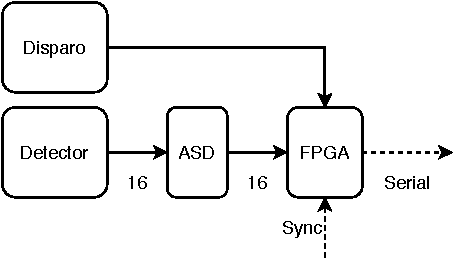
\includegraphics[scale=1]{imagenes/fpga1.pdf}
    \caption{Diagrama de bloques utilizando una FPGA como alternativa de solución. Se indica una salida serial para transmitir los resultados del análisis básico a algún procesador o memoria de alguna etapa posterior. La señal de sincronización, inspirada en la alternativa \ref{sec:micro} tiene como objetivo sincronizar la recolección y procesamiento de eventos, para que estos sean consistentes entre detectores.}
    \label{fig:fpga1}
\end{figure}

\begin{figure}[H]
    \centering
    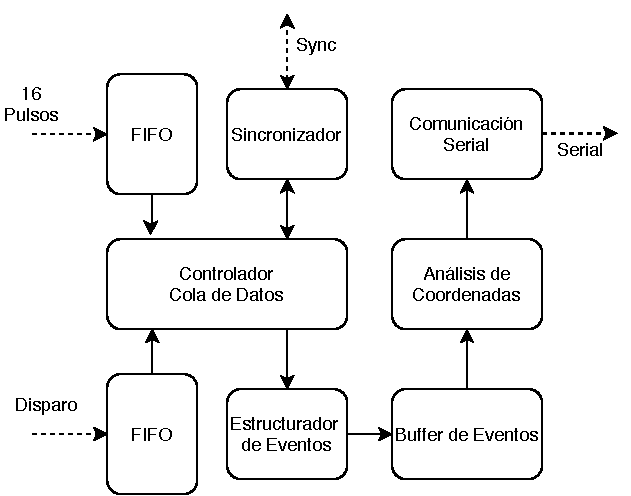
\includegraphics[scale=1]{imagenes/fpga2.pdf}
    \caption{Representación de la lógica interna de la FPGA. Se agrega una cola de datos para las señales de disparo y una memoria de almacenamiento temporal para los eventos ya estructurados. Ambas implementaciones permiten tener mejor control del flujo de datos, evitando perdidas y asegurando sincronía a pesar de que la lectura de la información sea eventualmente más lenta que la captura de pulsos. Los bloques controlador, estructurador y análisis cumplen las mismas funciones mencionadas en alternativas anteriores: aceptar o descartar pulsos, cuantificar anchos de pulso a  los canales asociados y determinar coordenada del cruce de un muón respectivamente.}
    \label{fig:fpga2}
\end{figure}

\newpage
\subsubsection*{Atributos}
\begin{itemize}
    \item \textbf{Simplicidad:}  Media. Gran cantidad del sistema concentrado en una sola placa, pero aumenta la dificultad en la descripción de hardware.
    \item \textbf{Desempeño:}  Alto. Gran cantidad de recursos lógicos, de almacenaiento y de frecuencia de operación.
    \item \textbf{Disponibilidad: } Alta. Se cuenta con una en el laboratorio.
    \item \textbf{Economía: } Media. Una tarjeta de desarrollo de este estilo tiene un costo de aproximadamente US\$400.
\end{itemize}

\subsubsection*{Ventajas}
\begin{itemize}
    \item Gran cantidad del sistema concentrado en una sola placa.
    \item Escalable
    \item Cuenta con puertos LVDS
    \item Alta densidad de recursos lógicos
    \item Dispone de memoria suficiente para almacenar eventos
    \item Posee una alta frecuencia de reloj sintetizable, mejorando precisión temporal.
    \item Placa con muy buena documentación.
\end{itemize}


\subsubsection*{Desventajas}
\begin{itemize}
    \item Se requiere confeccionar un adaptador para conectar el detector con la tarjeta de desarrollo.
    \item Se complica el diseño y la implementación del hardware.
\end{itemize}




\newpage
\section{Conclusiones}
\par Luego de estudiar cuatro alternativas de solución, es posible aseverar que una FPGA cuenta con la mayor capacidad para cumplir con los objetivos de este proyecto.
\par Si bien otras alternativas pueden tener ventajas en cuanto a precio, una FPGA simplifica algunas labores y da la holgura necesaria para implementar el sistema descrito.
\par Una quinta alternativa muy interesante es la utilización de una FPGA en conjunto con un procesador, como es el caso de las Zynq, mencionadas en informes anteriores. Estos dispositivos no fueron considerados ya que en el laboratorio no se encuentran disponibles tarjetas de desarrollo que cumplan con las especificaciones planteadas, particularmente con el número de puertos LVDS accesibles y necesarios para la confección del detector.
\par Otra alternativa descartada ha sido la aplicación de TDC (Time to Digital Converter)\cite{Arpin2010AResources}, que si bien permitiría mejorar la resolución temporal del sistema, implica un desafío ingenierily de recursos a una escala un tanto mayor.
\par Estas dos últimas propuestas quedan disponibles para ser implementadas en iteraciones posteriores, una vez que se tenga certeza del funcionamiento básico requerido que el actual proyecto plantea.

%
%\newpage
%\thispagestyle{empty}
%\cleardoublepage
%
%\chapter{Selección de Alternativa}
%\label{cap:selection}
%\par En el documento ``Alternativas de Solución de Proyecto de Titulación''\cite{Gonzalez2020AlternativasTitulacion} se presentaron 4 posibles alternativas para la implementación de un sistema de adquisición de datos para detectores de muones. En cada una de ellas se proponen distintas tecnologías para llevar acabo el mismo fin: Digitizers, Microcontroladores, CPLDs y FPGAs. La figura \ref{fig:diagrama} ilustra la estructura general del sistema de adquisicón de datos. 
\par En el actual documento se presenta el contraste entre las 4 alternativas discutidas con anterioridad, asignando puntaciones a cada una de ellas en base a criterios clave asociados a las características y el diseño del sistema. Los criterios a evaluar son: simplicidad, desempeño, disponibilidad, economía, flexibilidad y documentación. La comparativa que se desarrolla aquí tiene como objetivo definir cuál de las 4 opciones es la mejor alternativa a desarrollar, cumpliendo además con los requisitos principales del proyecto.
\par La alternativa seleccionada se presenta y detalla a continuación de la comparación de alternativas, planteando sus características principales y justificando la elección realizada.
%\begin{figure}[H]
%    \centering
%    
%    \tikzstyle{externo} = [rectangle, rounded corners, minimum width=2cm, minimum height=1cm,text centered, draw=black, fill=blue!30]
%    \tikzstyle{fpga} = [rectangle, rounded corners, minimum width=3cm, minimum height=2.5cm,text centered, draw=black, fill=green!30]
%    \tikzstyle{flecha} = [thick,->,>=stealth]   
%    
%    \begin{tikzpicture}[node distance=1.5cm]
%
%        \node (disparo) [externo] {Disparo};
%        \node (detector) [externo, below of=disparo] {Detector};
%        \node (asd) [externo, right of=detector, xshift=1cm] {ASD};
%        \node (disc) [fpga, right of=detector, xshift=2.5cm, yshift=-0.5cm, anchor=south west] {Discriminador};
%        \node (pros) [fpga, right of=disc, xshift=2cm] {Procesamiento};
%        \node (res) [fpga, right of=pros, xshift=2cm] {Análisis};
%        
%        \draw [flecha] (disparo) --  (disc.west |- disparo);
%        \draw [flecha] (detector) -- (asd);
%        \draw [flecha] (asd) -- (disc.west |- asd);
%        \draw [flecha] (disc) -- (pros);
%        \draw [flecha] (pros) -- (res);
%
%    \end{tikzpicture}
%
%    \caption{Diagrama de bloques del sistema. En azul se presentan las etapas previas al proyecto que ya se encuentran desarrolladas y sobre las cuales no se tiene control. En verde se ilustran las etapas pendientes y que pueden ser desarrolladas en este proyecto. El disparo corresponde a la señal digital que indica si la partícula detectada es un muón y el ASD es un acondicionador de señal que genera pulsos digitales a partir de los pulsos analógicos captados.}
%    \label{fig:diagrama}
%\end{figure}


\section{Criterios de Selección}
\par Para seleccionar la alternativa más adecuada se definieron seis distintos criterios de evaluación, cada uno de los cuales puede obtener un puntaje entre 1 y 10. Los criterios tienen distinta relevancia dentro del proyecto, resultando en que algunos de ellos tengan mayor ponderación respecto a otros. La tabla \ref{tab:criterios} indica el porcentaje de relevancia correspondiente cada criterio de selección. 

\begin{table}[H]
\centering
\begin{tabular}{|l|c|}
\hline
\textbf{Criterio de Selección} & \textbf{Porcentaje de Relevancia} \\ \hline
Simplicidad & 10\% \\ \hline
Desempeño & 35\% \\ \hline
Disponibilidad & 25\% \\ \hline
Economía & 10\% \\ \hline
Flexibilidad & 10\% \\ \hline
Documentación & 10\% \\ \hline
\textit{Total} & \textit{100\%} \\ \hline
\end{tabular}
\caption{Porcentaje de relevancia para cada criterio.}
\label{tab:criterios}
\end{table}

\newpage
\par Se considera como criterio de mayor importancia al \textit{desempeño} estimado de la alternativa, ya que será el aspecto que defina la calidad y funcionamiento del sistema. En segundo lugar de relevancia se ubica la \textit{disponibilidad} de recursos, ya que sin ellos no es posible construir el dispositivo. Los criterios restantes se consideraron menor con ponderación ya que son importantes, pero no cruciales para llevar a cabo el proyecto en su primera versión.
\par Cada criterio es evaluado con un puntaje de 1 a 10 puntos en una escala indicada en la tabla \ref{tab:escala}. A continuación se detalla cada criterio, incluyendo su descripción y explicando la interpretación de puntaje según la escala mencionada.

\begin{table}[H]
\centering
\begin{tabular}{lllll}
\hline
\multicolumn{1}{|c|}{\textbf{Muy Baja}} & \multicolumn{1}{c|}{\textbf{Baja}} & \multicolumn{1}{c|}{\textbf{Media}} & \multicolumn{1}{c|}{\textbf{Alta}} & \multicolumn{1}{c|}{\textbf{Muy Alta}} \\ \hline
\multicolumn{1}{|c|}{1 - 2}                 & \multicolumn{1}{c|}{3 - 4}             & \multicolumn{1}{c|}{5 - 6}           & \multicolumn{1}{c|}{7 - 8}           & \multicolumn{1}{c|}{9 - 10}              \\ \hline 
\end{tabular}
\caption{Tabla de puntajes para criterios de evaluación.}
\label{tab:escala}
\end{table}

\subsection*{Simplicidad}
\par El criterio de simplicidad se refiere a la dificultad de diseñar, programar, fabricar y ensamblar el sistema descrito en la alternativa evaluada. La máxima simplicidad está indicada con un puntaje 10 y la mínima simplicidad con un puntaje 1. Máxima simplicidad implica conectar elementos sin mayor esfuerzo, prácticamente no programar software y prácticamente no diseñar ni implementar hardware. Mínima simplicidad implicaría dificultad de interconexión entre elementos componentes, debido a sus estándares o cantidad de conexiones presentes, incluyendo software de alta complejidad y prácticamente el desarrollo completo del hardware.

\subsection*{Desempeño}
La evaluación por desempeño tiene directa relación con los requisitos de diseño asociados al sistema a desarrollar. Estos requisitos son los siguientes:

\begin{itemize}
    \item Se debe contar con al menos 32 pares de entradas bajo el estándar LVDS, con el fin de conectar al menos 2 tarjetas ASD (Amplificator Shaper Discriminator) utilizadas cada una como la interfaz de detectores de 16 canales.
    \item Es importante contar con un reloj presente o sintetizable de una frecuencia mayor a 100[MHz], lo más cercano a 1[GHz] posible, con el fin de captar la duración de los pulsos y el momento de aparición de un evento con la mayor precisión disponible.
    \item Se debe considerar que la señal de disparo que entrará al sistema estará desfasada cerca de 100[ns] respecto al paso real de los muones por el detector, siendo necesaria la implementación de retardos para las señales capturadas o un sistema capaz de distinguir la ocurrencia de eventos y disparos en el tiempo.
    \item  Se debe tener la capacidad de mantener señales sincronizadas, guardar información en memorias temporales y llevar cuenta del transcurso del tiempo entre eventos.
    \item Es requisito que la implementación de la alternativa permita escalamiento para agregar nuevos detectores adyacentes con el fin de aumentar el área de prueba, así como también sincronizarse con detectores paralelos para trazar trayectorias de las partículas captadas.
\end{itemize}

\par Sintetizando estos requisitos, es posible acotarlos a  5 elementos esenciales: número de canales, disponibilidad de puertos LVDS, frecuencia de reloj, implementación o manejo de retardos y recursos de almacenamientos o procesamiento disponibles. La escalabilidad queda implícitamente evaluada con los criterios de simplicidad, economía y flexibilidad.

\par Considerando lo anterior, se le asignará puntaje a este criterio en función de la cantidad de requisitos que cumpla y la calidad con la que sean satisfechos, considerando 10 puntos en caso de cumplir a cabalidad con todos ellos, y asignándole 1 punto en caso de cumplir ninguno.

\subsection*{Disponibilidad}
\par El criterio de disponibilidad evalúa la presencia inmediata de los materiales necesarios para la implementación del sistema. Pondera la cantidad de elementos necesarios como un total de 10 puntos repartidos en cada uno de los elementos componentes para construir un sistema de adquisición de 32 canales. Si un sistema requiere de 5 elementos discretos, tendrá entonces 10 puntos en caso de contar con la disponibilidad de los 5 elementos necesarios. Si alguno no está disponible y requiere ser adquirido, entonces implicaría un descuento de 2 puntos en dicho ejemplo.

\subsection*{Economía}
\par El criterio de economía evalúa el precio total de construcción del dispositivo, incluyendo todo el hardware necesario para la discriminación, procesamiento y análisis, sin considerar un computador en las etapas finales de análisis o recolección de información. Este criterio es útil para contrastar la factibilidad de escalamiento. Un sistema muy costoso implicará dificultades para replicarlo.
\par Su puntaje se asigna considerando cero puntos para un sistema que supere los US\$1000 para implementar 32 canales. Se otorga un máximo de 10 puntos si el sistema tiene un costo menor o igual a US\$60.

\subsection*{Flexibilidad}
\par La flexibilidad es un criterio que representa qué tan adaptable es el sistema en caso de requerir modificaciones. Puede separarse en tres elementos constitutivos: adquisición, procesamiento y análisis. El puntaje se asigna cualitativamente en función de la flexibilidad de la tecnología involucrada en dicha etapa.
\par El puntaje máximo del criterio de flexibilidad son 10 puntos, considerando aproximadamente 3.3 puntos como máximo para cada elemento constitutivo.

\subsection*{Documentación}
\par El criterio de documentación evalúa la disponibilidad de material bibliográfico, tutoriales y ejemplos para la utilización del software y el hardware propio del sistema, así como de las herramientas necesarias para su implementación. Su puntaje se asigna cualitativamente según la misma tabla \ref{tab:escala}.

\newpage
\section{Evaluación de Alternativas}
\label{evaluacion}
\par A continuación se detallan las evaluaciones para cada una de las 4 alternativas propuestas, incluyendo una breve descripción por cada criterio.
\subsection{Digitizer}
\begin{itemize}
    \item \textbf{Simplicidad:} \textit{5 - Media}. Requiere la fabricación de una PCB de interfaz y la integración de 3 aparatos distintos (Digitalizador, interfaz y computador).
    \item \textbf{Desempeño:} \textit{4 - Bajo}. Baja tasa de muestreo, 62.5[MS/s].
    \item \textbf{Disponibilidad:} \textit{2 - Muy Baja}. Se cuenta con un digitalizador, pero no está disponible una interfaz LVDS a TTL ni los retardos necesarios.
    \item \textbf{Economía:} \textit{1 - Muy Baja}. El costo de  un  digitalizador podría superar los US\$1000.
    \item \textbf{Flexibilidad:} \textit{5 - Media}. Alta flexibilidad en análisis ya que se realiza en un computador. También existe flexibilidad en la manera de procesar y estructurar los datos obtenidos. No existe suficiente flexibilidad en la manera de tomar muestras.
    \item \textbf{Documentación:} \textit{6 - Media} Existe documentación, librerías y programas para operar el digitalizador, pero no son las suficientes para tener el dominio total del dispositivo.
\end{itemize}

\subsection{Microcontrolador}
\begin{itemize}
    \item \textbf{Simplicidad: } \textit{2 - Baja}. Gran cantidad de dispositivos, al ser necesario al menos dos microcontroladores por canal y un tercero para unificar datos provenientes de un mismo detector.
    \item \textbf{Desempeño: } \textit{4 - Bajo}. Bajas tasas de muestreo y operación. Requiere conversores LVDS-TTL y retardos.
    \item \textbf{Disponibilidad: } \textit{1 - Baja}. Todos los materiales tendrían que ser adquiridos.
    \item \textbf{Economía: } \textit{6 - Media}, medianamente económico. Si bien las tarjetas de desarrollo pueden ser de bajo costo, se necesitan varias y se agregan componentes extra que aumentan el costo considerablemente. Mejorar la frecuencia de muestreo también incrementa el costo.
    \item \textbf{Flexibilidad:} \textit{5 - Media}. Alta flexibilidad en análisis y en la manera de procesar y estructurar los datos obtenidos. No existe suficiente flexibilidad en la manera de tomar muestras.
    \item \textbf{Documentación:} \textit{6 - Media} Existe documentación, librerías y programas de ejemplo, pero queda sujeto a los microcontroladores que eventualmente se escojan.
\end{itemize}

\newpage
\subsection{CPLD}
\begin{itemize}
    \item \textbf{Simplicidad:} \textit{7 - Alta}. Pocos dispositivos involucrados, solo una CPLD por detector.
    \item \textbf{Desempeño:}  \textit{7 - Alto}. Escasos recursos lógicos y periféricos, pero alta velocidad de reloj (400MHz máximo), opciones para manejar ratardos y cuenta con puertos LVDS.
    \item \textbf{Disponibilidad:} \textit{9 - Alta}. Se cuenta con una de estas tarjetas en el laboratorio.
    \item \textbf{Economía: } \textit{10 - Alta}. Una de estas tarjetas tiene un valor cercano a los US\$30.
    \item \textbf{Flexibilidad:} \textit{10 - Alta}. Alta flexibilidad en análisis, procesamiento y adquisición.
    \item \textbf{Documentación:} \textit{4 - Baja} Existe documentación, pero es poca y no es simple. Existen pocos ejemplos en internet dado que es un fabricante menos conocido y poco aplicado en este tipo de desarrollos. La herramienta de descripción de hardware es similar a las conocidas, pero propia del fabricante.
\end{itemize}


\subsection{FPGA}
\begin{itemize}
    \item \textbf{Simplicidad:}  \textit{6 - Media}. Gran cantidad del sistema concentrado en una sola placa, pero aumenta la dificultad en la descripción de hardware.
    \item \textbf{Desempeño:}  \textit{9 - Alto}. Gran cantidad de recursos lógicos, de almacenamiento y con alta  frecuencia de operación (600MHz máximo).
    \item \textbf{Disponibilidad: } \textit{9 - Alta}. Se cuenta con una en el laboratorio, pero se necesitarán un par de elementos para interconectarla con la placa ASD.
    \item \textbf{Economía: }\textit{6 - Media}. Una tarjeta de desarrollo de este estilo tiene un costo de aproximadamente US\$400.
    \item \textbf{Flexibilidad:} \textit{10 - Alta}. Alta flexibilidad en análisis, procesamiento y adquisición.
    \item \textbf{Documentación:} \textit{8 - Alta} Existe gran cantidad de documentación del fabricante. Además, cuenta con una FPGA Artix 7 ampliamente conocida.
\end{itemize}

\par Finalmente, se resumen en la tabla \ref{tab:comparacion} los puntajes obtenidos por las alternativas propuestas en cada uno de los criterio de selección, acompañados de su puntaje final ponderado. De esta tabla se concluye que la alternativa a seleccionar será la FPGA, la cual obtuvo 8.4 puntos, superando a todas las demás alternativas. Esta alternativa destaca por su desempeño, disponibilidad y documentación.

\begin{table}[H]
\centering
\begin{tabular}{|l|c|c|c|c|}
\hline
\textbf{Criterio de Selección} & \textbf{Digitizer} & \textbf{Microcontrolador} & \textbf{CPLD} & \textbf{FPGA} \\ \hline
Simplicidad (10\%) & 5 & 2 & 7 & 6 \\ \hline
Desempeño (35\%) & 4 & 4 & 7 & 9 \\ \hline
Disponibilidad (25\%) & 2 & 1 & 9 & 9 \\ \hline
Economía (10\%) & 1 & 6 & 10 & 6 \\ \hline
Flexibilidad (10\%) & 5 & 5 & 10 & 10 \\ \hline
Documentación (10\%) & 6 & 6 & 4 & 8 \\ \hline
\textit{Total} & \textit{3.6} & \textit{3.55} & \textit{7.8} & \textit{8.4} \\ \hline
\end{tabular}
\caption{Comparación entre evaluaciones de cada alternativa propuesta.}
\label{tab:comparacion}
\end{table}


\section{Alternativa Seleccionada}
\label{alternativa}

\par A partir de las evaluaciones indicadas en la sección \ref{evaluacion} y sus comparaciones en la tabla \ref{tab:comparacion}, se concluye que la mejor alternativa corresponde a un sistema de adquisición de datos implementado en una FPGA (Artix 7\cite{Xilinx20107DS180}).
\par Esta alternativa fue seleccionada por sobre las demás debido a su destacado desempeño, ya que cuenta con mayor frecuencia de reloj disponible, gran cantidad de recursos y suficientes puertos LVDS. Este último requerimiento es necesario para recibir los pulsos digitales capturados por la interfaz ASD\cite{1999ATLASICs} provenientes del detector, los cuales se emiten bajo el estándar LVDS para transmisión de señales diferenciales.
\par Destaca también esta alternativa al ser una plataforma flexible, en sentido de brindar las posibilidades de adaptar el diseño propuesto sin tener que adquirir nuevo equipamiento. Esta versatilidad es intrínseca de las FPGAs, las cuales se caracterizan por permitir un gran control en el diseño del hardware a bajo nivel.
\par Por último, destaca por la información disponible que existe para operarla. Esta FPGA es ampliamente conocida y además está incluida en un módulo Trenz TR0712\cite{TrenzElectronic2019TR07012Wiki} montada en una tarjeta Trenz TR0703\cite{TrenzElectronic2019TR0703Wiki} que da acceso a la mayoría de sus puertos y recursos. Ambos elementos cuentan con buena documentación, incluyendo diagramas de conexiones detallados, los cuales facilitarán la descripción del hardware y la interconexión con el detector de muones.

\begin{figure}[H]
    \centering
    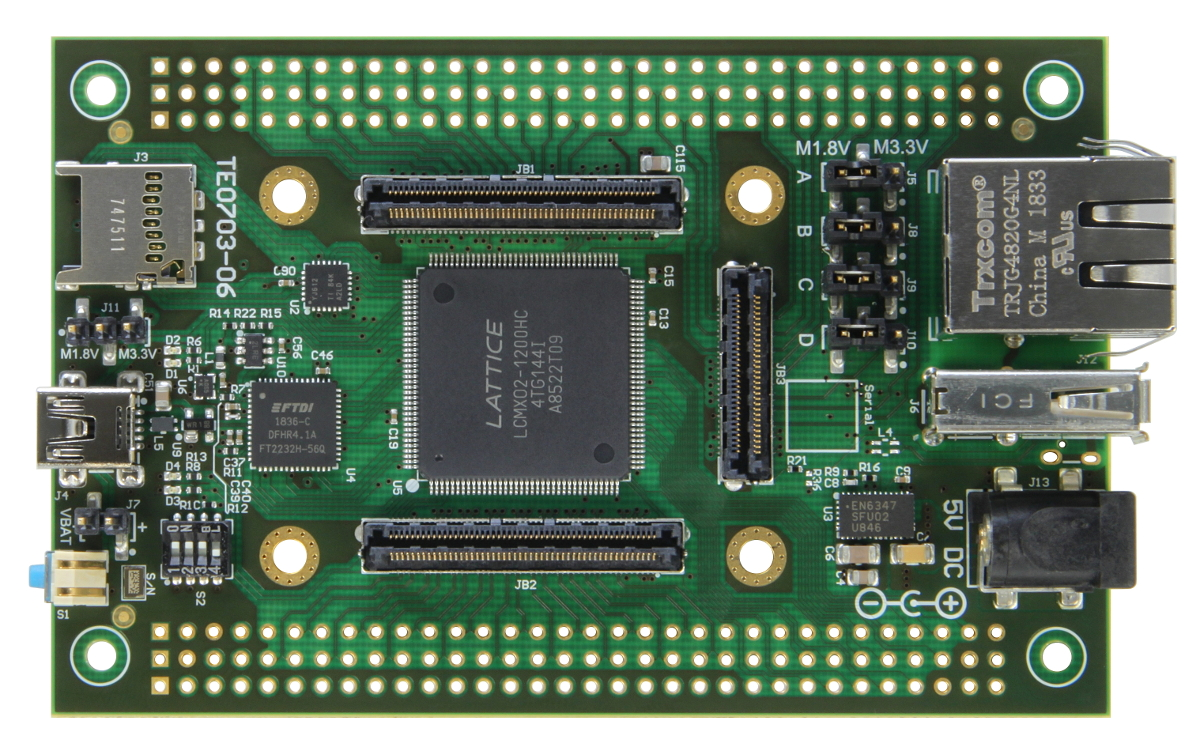
\includegraphics[scale=0.23]{imagenes/TE0703-06_1.jpg}
    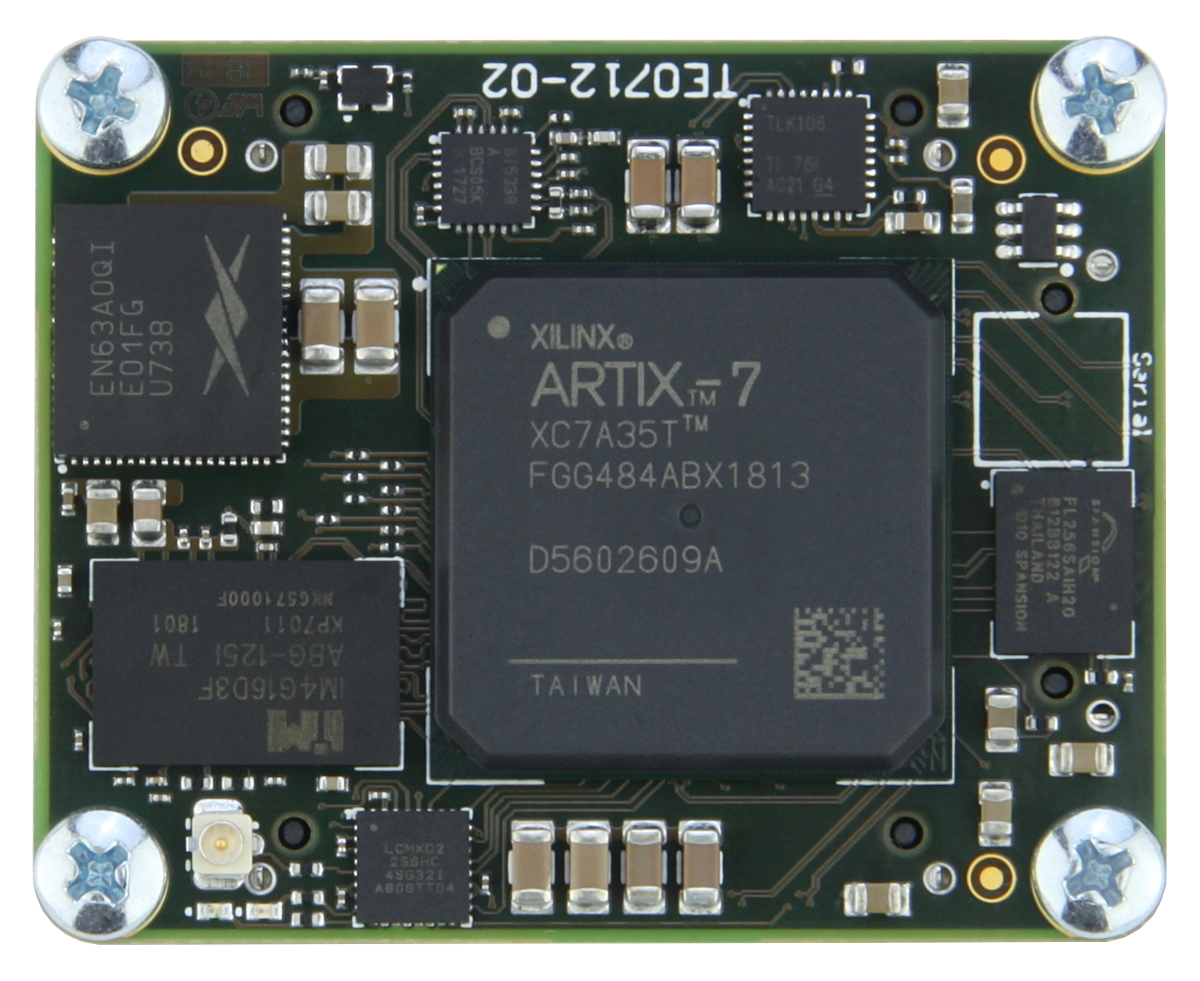
\includegraphics[scale=0.13]{imagenes/TE0712-02-35-2I_1.jpg}
    \caption{Placa de desarrollo y módulo FPGA a utilizar. A la izquierda se ilustra la placa de desarrollo Trenz TR0703\cite{TrenzElectronic2019TR0703Wiki} y a su derecha se ilustra el módulo que va montado en ella: Trenz TR0712\cite{TrenzElectronic2019TR07012Wiki} que contiene una FPGA Artix 7\cite{Xilinx20107DS180}.}
    \label{fig:trenz}
\end{figure}


\par Para esta alternativa de solución se consideran 32 canales de entrada LVDS ya que en el futuro será necesario conectar al menos 2 detectores de 16 canales en una misma FPGA. Para este proyecto en particular se probará el sistema con un solo detector de muones, por lo que la prueba e integración de un segundo detector queda pendiente y no se implementará en esta etapa. La figura \ref{fig:ministgc} ilustra los canales que posee un solo detector de muones de $15cm^2$.

\begin{figure}[H]
    \centering
    \includegraphics[scale=0.5]{imagenes/ministgc.pdf}
    \caption{Esquema de los canales provenientes de un detector Mini sTGC. Posee 8 tiras adyacentes de 15cm de largo por 1cm de ancho para cada eje coordenado. Cada tira emitirá un pulso analógico si una partícula cargada pasa través de ella. Se emitirán también pulsos de menor amplitud para el caso en que la partícula pase por una tira adyacente del mismo eje coordenado dentro de un radio específico. Este detector se posiciona perpendicularmente respecto a la fuente de radiación y en paralelo a (por debajo o por sobre) el sistema de disparo que indicará si la partícula captada corresponde o no a un muón. }
    \label{fig:ministgc}
\end{figure}

\par Las señales generadas por un detector son adaptadas por una tarjeta de interfaz ASD\cite{1999ATLASICs}, ilustrada en la figura \ref{fig:asd}. Esta tarjeta es capaz de capturar 16 señales simultaneas, por lo que es hardware suficiente para captar las señales de ambos ejes de un solo detector de muones.

\begin{figure}[H]
    \centering
    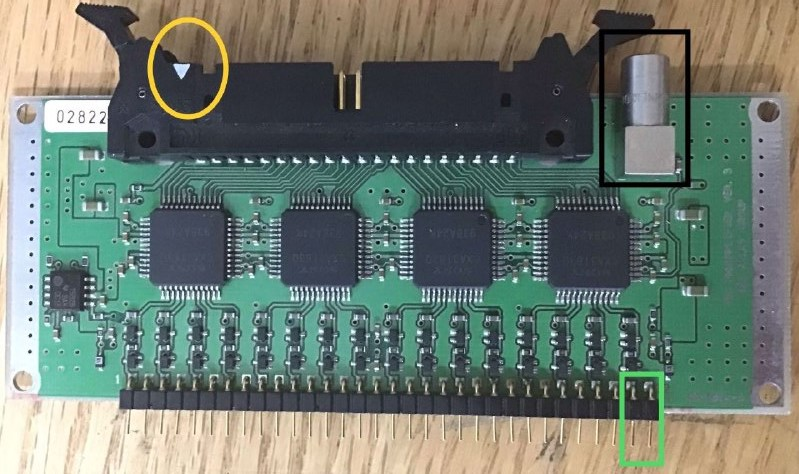
\includegraphics[scale=0.4]{imagenes/asd.jpg}
    \caption{Placa ASD\cite{1999ATLASICs} (Amplificator Shaper Discriminator), encargada de captar los 16 pulsos provenientes de un detector y entregar pulsos digitales asociados a ellos en su salida. El detector se conecta en sus entradas DIP ubicadas en su extremo inferior, mientras que las señales LVDS de salida se ubican en el conector de 40 puertos para cable plano en su extremo superior.}
    \label{fig:asd}
\end{figure}

\begin{figure}[H]
    \centering
    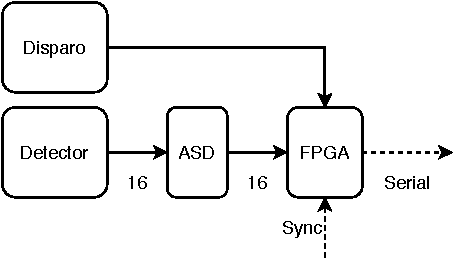
\includegraphics[scale=0.75]{imagenes/fpga1.pdf}
    \caption{Diagrama de bloques utilizando una FPGA como alternativa de solución. Se indica una salida serial para transmitir los resultados del análisis básico a algún procesador o memoria de alguna etapa posterior. La señal de sincronización ``Sync'' tiene como objetivo sincronizar la recolección y procesamiento de eventos, para que estos sean consistentes entre detectores.}
    \label{fig:fpga1}
\end{figure}


\par La idea en esta alternativa de solución es guardar los pulsos provenientes de la placa ASD en memoria temporal hasta la llegada de una señal de disparo. Un módulo que maneja la memoria será el encargado de tomar los pulsos correspondientes al disparo recibido y liberar la memoria de aquellos datos ya leídos u obsoletos, entregando la información útil a una siguiente etapa. Los pulsos aceptados serán entonces relacionados como parte de un mismo eventos y se estimará la duración de estos, generando y guardando así un arreglo de datos con identificador de pulso y duración. La última etapa se encargará de efectuar una operación capaz de determinar la posición del evento a partir de las duraciones medidas y los pulsos detectados, comunicando así un arreglo básico y preprocesado que incluya posición espacial y magnitud aproximada.


\begin{figure}[H]
    \centering
    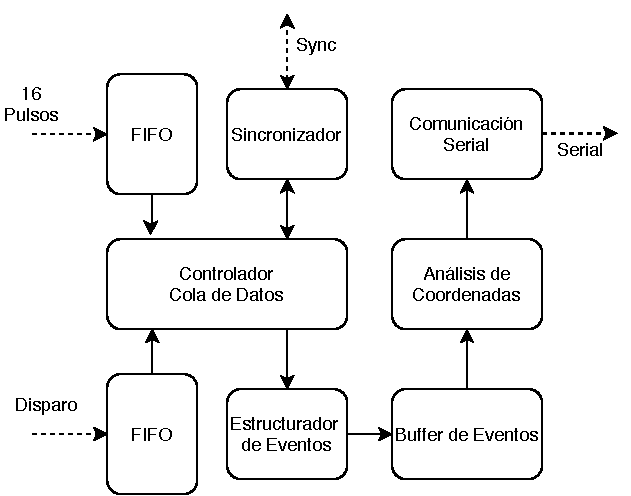
\includegraphics[scale=0.75]{imagenes/fpga2.pdf}
    \caption{Representación de la lógica interna de la FPGA. Se incluye una cola de datos para las señales de disparo, para los pulsos digitales provenientes de la ASD y una memoria de almacenamiento temporal para los eventos ya estructurados. Los bloques controlador, estructurador y análisis cumplen las funciones de aceptar o descartar pulsos, cuantificar anchos de pulso a  los canales asociados y determinar coordenada del cruce de un muón respectivamente.}
    \label{fig:fpga2}
\end{figure}

\par Se espera que para lograr el escalamiento se incluya una señal para mantener la lectura de eventos sincronizada entre distintas FPGA. Además, se deberá incluir un modulo de comunicación para entregar la información captada a una etapa posterior con un análisis más detallado, encargado de reunir todos los eventos de diferentes FPGAs.


\newpage
\section{Conclusión}
\par Luego de presentar y evaluar diferentes alternativas de solución, el análisis indica que la mejor solución corresponde a implementar el sistema en una FPGA, obteniendo un resultado de 8.4 puntos según los criterios de selección. Esta alternativa fue precisamente la que se ha considerado desde un principio y coincide con ser la tecnología más utilizada dentro del desarrollo de sistemas de adquisición para física de partículas\cite{Basiladze2017Methods1}\cite{Basiladze2017Methods2}.
\par Esta alternativa fue seleccionada por sobre las demás debido a su destacado desempeño, ya que cuenta con mayor frecuencia de reloj disponible, gran cantidad de recursos y suficientes puertos LVDS. Este último requerimiento es necesario para recibir los pulsos digitales capturados por la interfaz ASD provenientes del detector, los cuales se emiten bajo el estándar LVDS para transmisión de señales diferenciales.
\par Destaca también esta alternativa al ser una plataforma flexible, en sentido de brindar las posibilidades de adaptar el diseño propuesto sin tener que adquirir nuevo equipamiento. Esta versatilidad es intrínseca de las FPGAs, las cuales se caracterizan por permitir un gran control en el diseño del hardware a bajo nivel.
\par Luego de este trabajo de selección y detalle de la solución, ya se encuentran definidos los objetivos principales del proyecto y los esquemas generales del diseño a implementar para cumplir con ellos. Con la información presentada en la sección \ref{alternativa} es posible comenzar las etapas de planificación y posterior ejecución del proyecto, para desarrollar así un sistema de adquisición de datos para detectores de muones escalable basado en FPGA.

%
%\newpage
%\thispagestyle{empty}
%\cleardoublepage

\chapter{Detección}
\label{cap:stgc}

La detección de muones en este proyecto es realizada mediante un detector de partículas inspirado en los detectores sTGC del proyecto ATLAS, en CERN. La sigla significa ''small Thin Gap Chamber", y forman parte de un espectrómetro de muones que permite conocer momento y trayectoria de estas partículas. Los muones proveen de información importante para la reconstrucción de eventos asociados a colisiones de partículas.

\begin{figure}[h]
	\centering
	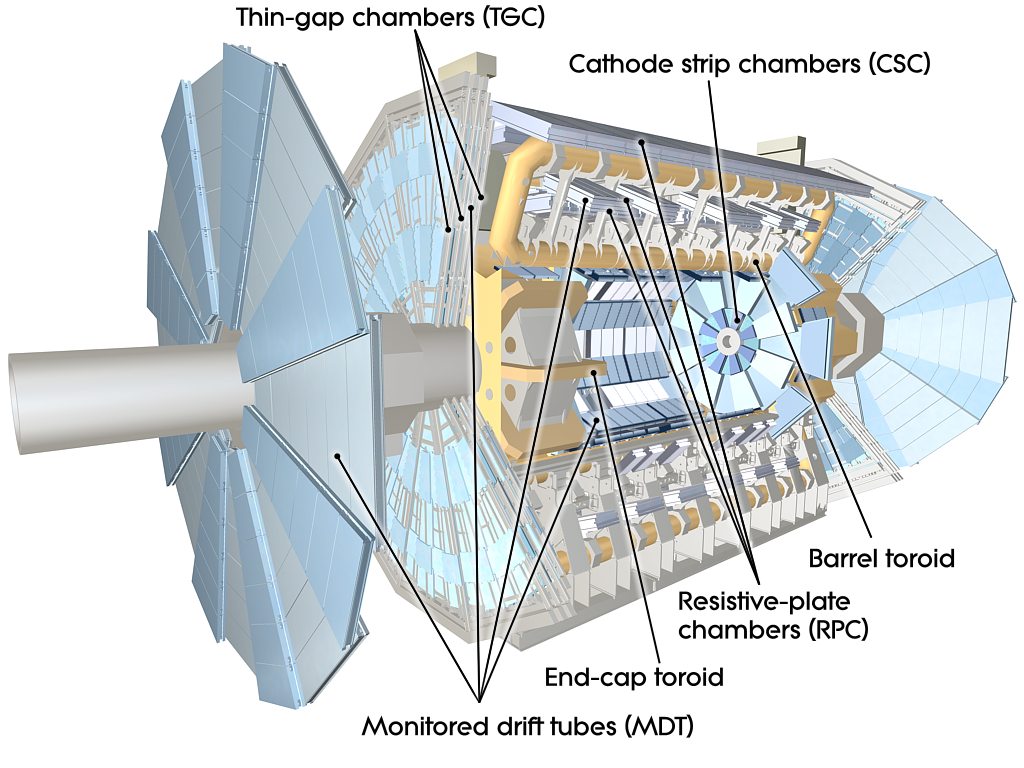
\includegraphics[scale=0.3]{atlas-muon-spectrometer-layout.png}
	\caption{Diagrama del espectrómetro de muones en el proyecto ATLAS\cite{AtlasMuonDiagram}.}
	\label{img:atlas-layout}
\end{figure}

\newpage
\begin{figure}[h]
	\centering
	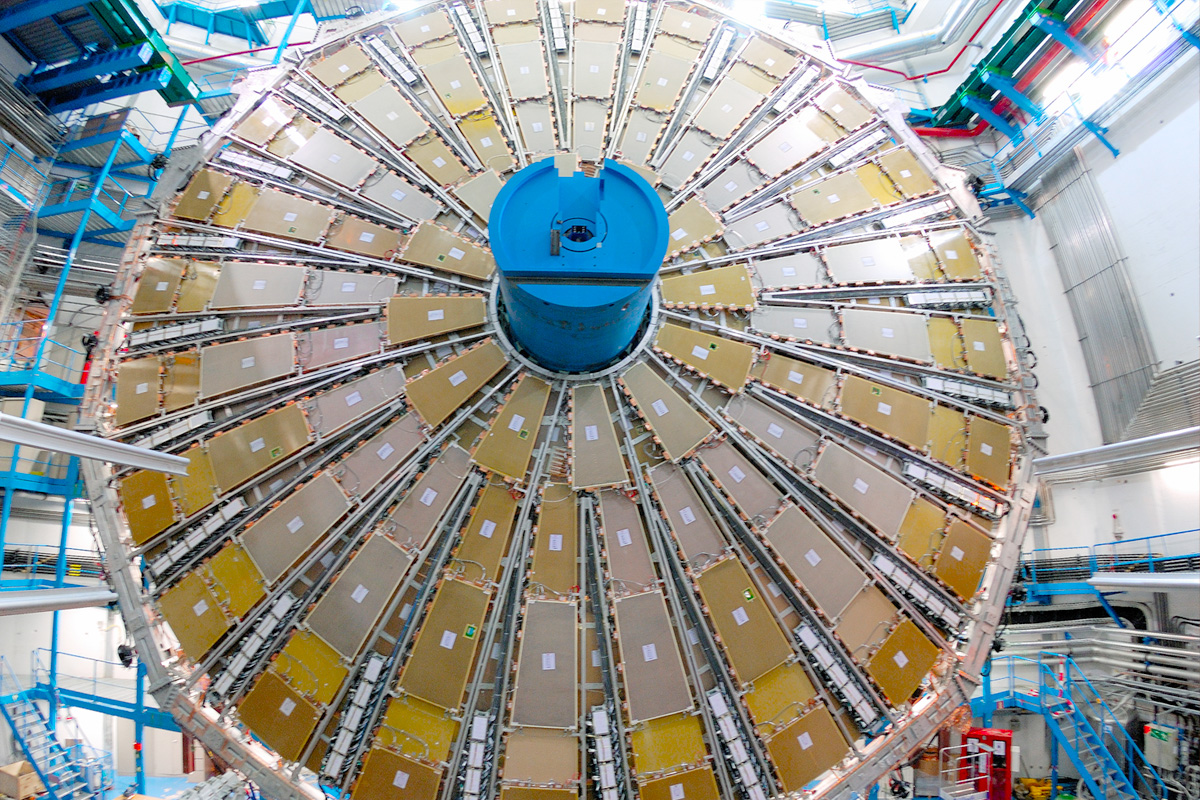
\includegraphics[scale=0.3]{atlas-muon-tgc.jpg}
	\caption{Fotografía del los detectores sTGC en el espectrómetro de muones del proyecto ATLAS\cite{AtlasMuonSpect}.}
	\label{img:atlas-tgc}
\end{figure}

\begin{figure}[h]
	\centering
	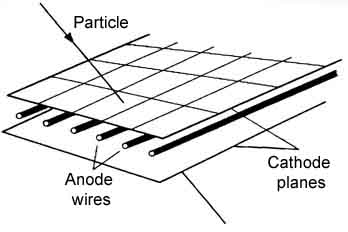
\includegraphics[scale=1]{stgc-lateral.jpg}
	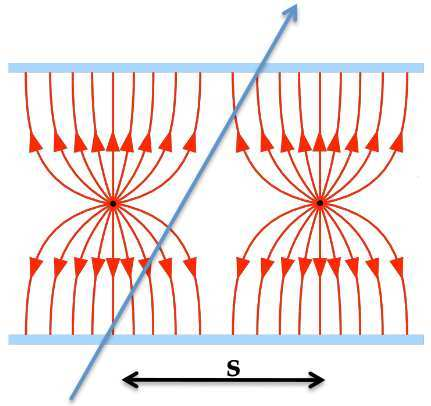
\includegraphics[scale=0.3]{stgc-transversal.png}
	\caption{Esquemas de un detector. La figura izquierda representa una vista lateral, mientras que la derecha ilustra un corte transversal del mismo. En ambos se observan  }
	\label{img:stgc-diagrams}
\end{figure}

\newpage
\subsection*{Estructura}

	Un TGC se compone de dos planos catódicos y varios cables anódicos. Los cátodos están seccionados en tiras llamadas "\textit{strips}". Los cables se encuentran ubicados perpendicularmente respecto a los \textit{strips}.
	
	Al interior del detector, entre los planos catódicos, se infiltra un gas compuesto por dióxido de carbono y pentano. Mediante la aplicación de alto voltaje, se genera un campo eléctrico entre ánodos y cátodos.
	
	El paso de muones a través del detector genera la ionización del gas y la liberación de electrones que son captados por los cables del detector. Este flujo de electrones genera pulsos de corriente tanto en los \textit{strips} como en los cables. Estos pulsos son de mayor amplitud en torno a la zona del evento ionizante, mientras que a mayor distancia la amplitud disminuye. Esto permite relacionar la posición y energía de la partícula con las amplitudes de los pulsos en cada \textit{strip} o cable.

\subsection*{Mini sTGC Utilizado}
	En ATLAS se leen tanto cátodos como ánodos. Esto permite trazar cuadrantes de posición del evento, ya que los \textit{strips} son perpendiculares a los cables. En este proyecto de titulación se leerán solo las señales provenientes de los \textit{strips} catódicos, por los que solo se mide un eje de posición. 
	
	Para agregar un eje adicional, se superpone un segundo TGC con \textit{strips} perpendiculares al detector anterior. Así se puede tener información bidimensional del paso de una partícula leyendo solo los cátodos. De este modo, el detector utilizado para este proyecto de titulación corresponde a dos mini-detectores TGC superpuestos, con \textit{strips} perpendiculares entre sí.
	
	\begin{figure}
		\centering
		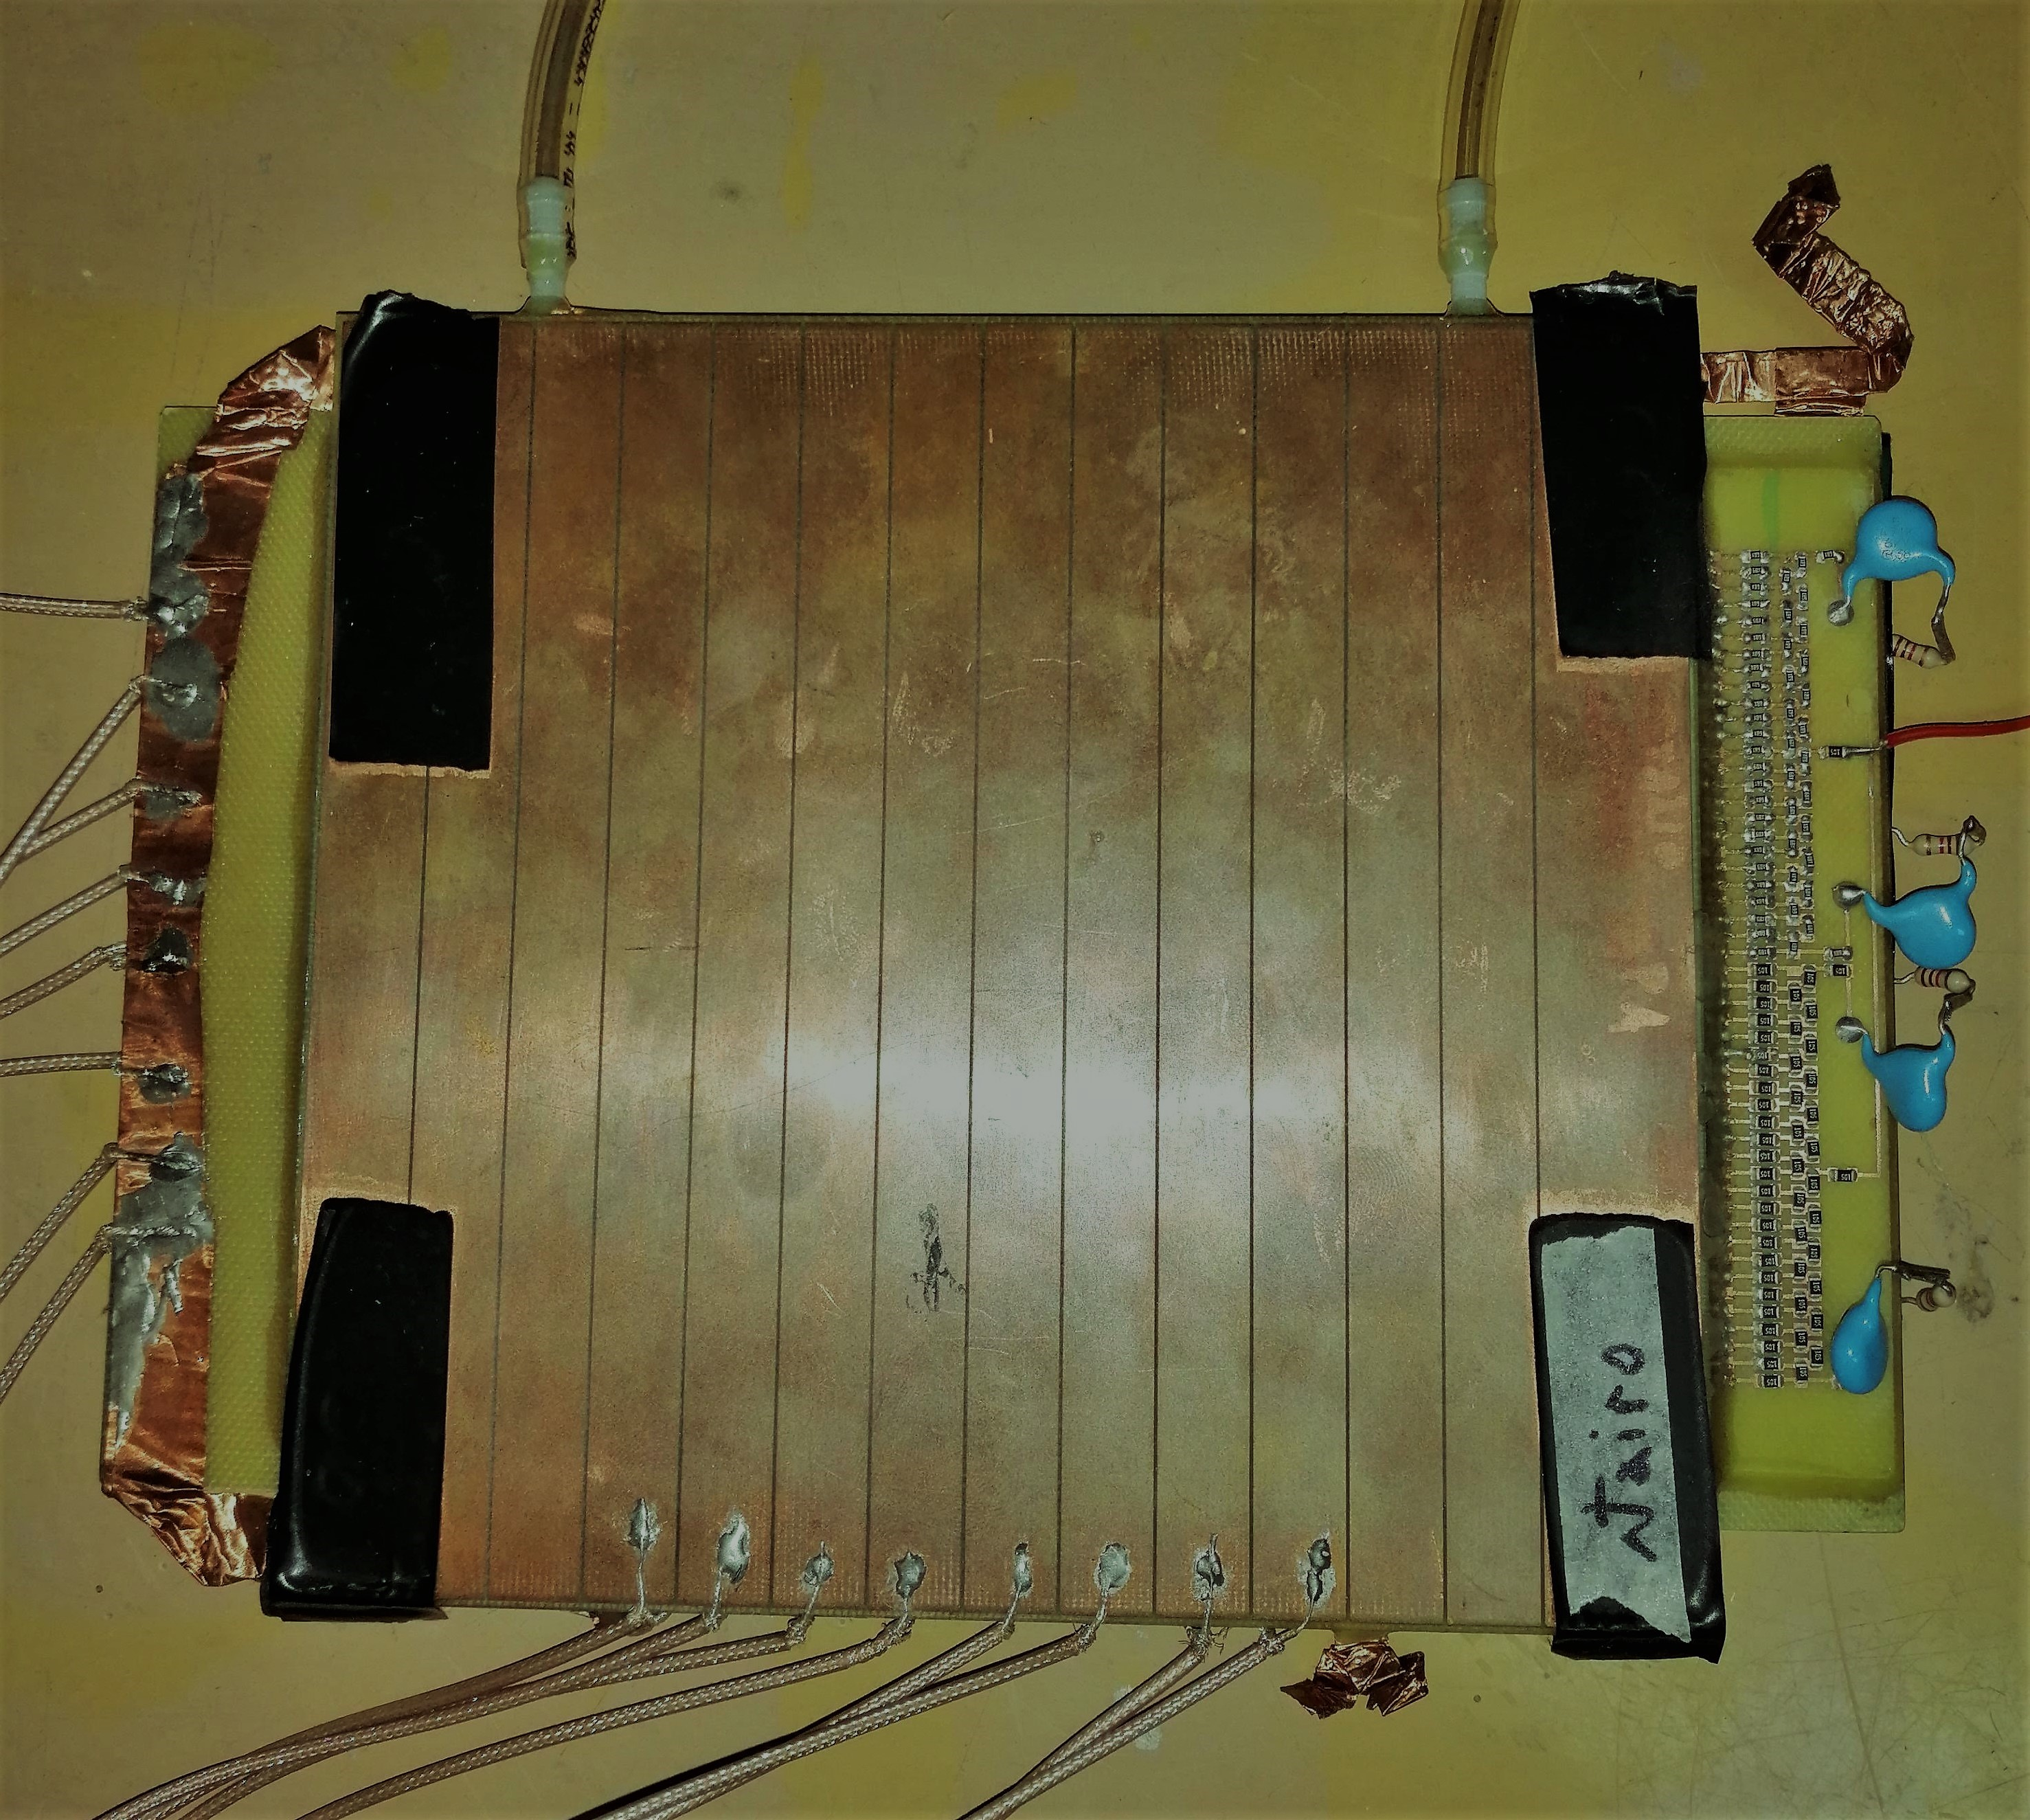
\includegraphics[scale=0.1]{mini-stgc.jpg}
		\caption{Vista superior del detector utilizado. Arriba se observan tubos para el flujo de gas. Abajo se ubican 8 cables coaxiales conectados a los \textit{strips} centrales de una cara del detector. A la izquierda están situados los otros 8 cables correspondientes a los \textit{strips} de la cara inferior. En el costado derecho se observa una red resistiva ponderadora para la lectura de los cables internos del detector, los cuales no serán utilizados en este proyecto.}
		\label{img:foto-mini-stgc}
	\end{figure}
	
	En particular, el detector utilizado cuenta con 8 \textit{strips} útiles, de 15 centímetros largo y 1 centímetro de ancho por cada sub-detector. El gas se ioniza con 3000VDC y una corriente límite de 50uA. El gas en su interior puede ser dióxido de carbono puro, con el compromiso de generar mayor cantidad de descargas no asociadas a muones.


%pruebas, gráficos, entradas y salidas, triggers, plásticos, fuentes radioactivas

%\newpage
%\thispagestyle{empty}
%\cleardoublepage
%
%\chapter{Lectura}
%\label{cap:asd}
%\input{6_Lectura.tex}
%
%\newpage
%\thispagestyle{empty}
%\cleardoublepage
%
%\chapter{Muestreo}
%\label{cap:samplig}
%\input{7_Muestreo.tex}
%
%\newpage
%\thispagestyle{empty}
%\cleardoublepage
%
%\chapter{Discriminación}
%\label{cap:discriminator}
%\input{8_Discriminacion.tex}
%
%\newpage
%\thispagestyle{empty}
%\cleardoublepage
%
%\chapter{Estructuración}
%\label{cap:structure}
%\input{9_Estructuracion.tex}
%
%\newpage
%\thispagestyle{empty}
%\cleardoublepage
%
%
%\chapter{Análisis}
%\label{cap:analysis}
%\input{10_Analisis.tex}
%
%\newpage
%\thispagestyle{empty}
%\cleardoublepage
%
%\chapter{Sincronización}
%\label{cap:sync}
%\input{11_Sincronizacion.tex}
%
%\newpage
%\thispagestyle{empty}
%\cleardoublepage
%
%\chapter{Comunicación}
%\label{cap:comm}
%\input{12_Comunicacion.tex}
%
%\newpage
%\thispagestyle{empty}
%\cleardoublepage
%
%\chapter{Pruebas}
%\label{cap:test}
%\input{13_Comunicacion.tex}
%
%\newpage
%\thispagestyle{empty}
%\cleardoublepage
%
%\chapter{Resultados}
%\label{cap:insights}
%\input{14_Resultados.tex}
%
%\newpage
%\thispagestyle{empty}
%\cleardoublepage
%
%\chapter{Conclusiones}
%\label{cap:conclusiones}
%\input{15_Conclusiones.tex}
%
%\newpage
%\thispagestyle{empty}
%\cleardoublepage
%
%%%%%%%%%%%%%%%%%%%%%%%%%%%%%%%%%%%%%%%%%%%%%%%%%%%%%%%%%%%%
%%%
%%%%------------------APÉNDICES--------------------------------
%%%
%%%%%%%%%%%%%%%%%%%%%%%%%%%%%%%%%%%%%%%%%%%%%%%%%%%%%%%%%%%%
%
%\appendix
%\chapter{Control de versiones de proyectos Vivado con Git}
%\label{git}
%\textit{Git} es un sistema de control de versiones que permite al desarrollador crear múltiples ramas de desarrollo, sincronizar su trabajo con otros desarrolladores, revertir cambios realizados en el código y mantener una versión ordenada de un proyecto. Usar este tipo de herramientas para el desarrollo de proyectos en Vivado Desing Suite resulta ser muy útil, ya que permite trabajar de manera colaborativa y llevar registro de las versiones del hardware diseñado. En este apéndice se resumen todos los consejos y etapas para llevar a cabo el control de versiones de un proyecto Vivado. La clave del método a describir consiste subir al repositorio solo los archivos principales del proyecto, dejando fuera cualquier otro archivo proveniente de etapas de síntesis, implementación o archivos generados automáticamente por Vivado. Para llevar a cabo el control de versiones se hace uso de \textit{git} en junto con la plataforma en línea \textit{Github.com}.

Antes de comenzar, se debe contar con los siguientes requisitos:
\begin{itemize}
	\item Nociones básicas de \textit{git}.
	\item Una cuenta en \textit{Github.com}.
	\item El software de control de versiones \textit{git} instalado en el computador y habilitado para ser operado mediante un terminal de comandos.
	\item Tener instalado Vivado Design Suite (La versión utilizada en este tutorial corresponde a la versión 2019.1).
\end{itemize}

\section{Creación de un repositorio Git}

	Para comenzar, se debe iniciar sesión en \textit{Github.com} y hacer clic en el botón verde  ``New'' ubicado en la esquina superior izquierda, como se ilustra en la Figura \ref{fig:git1}.
	
	\begin{figure}[ht]
		\centering
		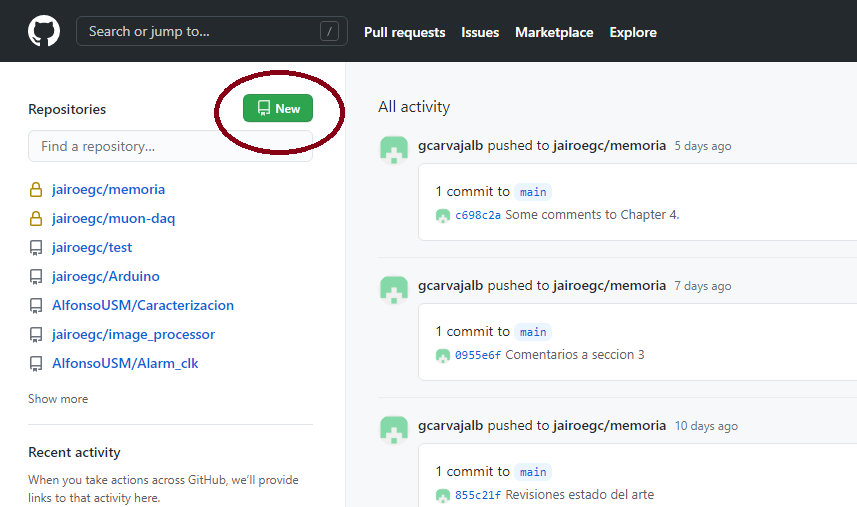
\includegraphics[scale=0.6]{git1.png}
		\caption{Botón ``New'' para la creación de un nuevo repositorio remoto en \textit{Github.com}.}
		\label{fig:git1}
	\end{figure}
	
	Se debe elegir el nombre del repositorio y configurar lo esencial. Se recomienda crear un proyecto en blanco, sin archivo \textit{readme} o \textit{.gitignore}, ya que serán subidos al repositorio de manera remota durante el primer \textit{commit}.

\section{Clonación de un repositorio Git}

	Desde la interfaz web del repositorio de Github.com debe buscarse el botón verde llamado ``Code'' (ubicado en la esquina superior derecha) y copiar en el portapapeles la \textit{URL} disponible para clonar el repositorio mediante HTTPS (Hypertext Transfer Protocol Secure), como se ilustra en la Figura \ref{fig:git2}.
	
	\begin{figure}[ht]
		\centering
		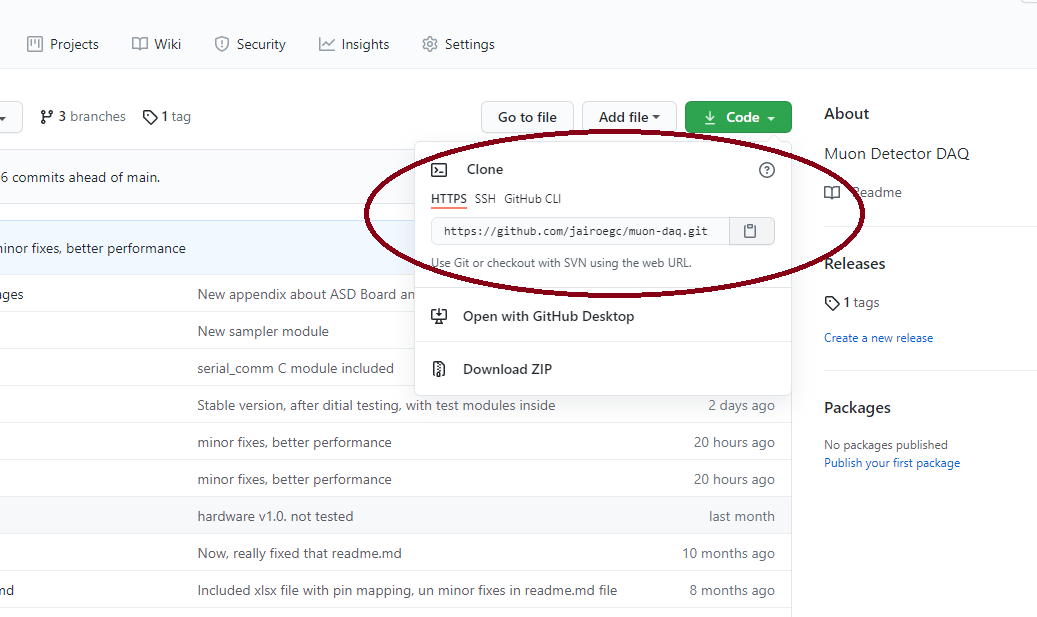
\includegraphics[scale=0.5]{git2.png}
		\caption{Botón ``Code'' para acceder al enlace de clonación del repositorio.}
		\label{fig:git2}
	\end{figure}
	
	Si aún no se tiene instalado \textit{git} en el computador, se debe proceder a su instalación vía consola o mediante descarga directa. Luego, se debe acceder o crear una carpeta para guardar el repositorio Vivado, abrir en ella una consola de comandos y escribir lo siguiente, sustituyendo \textit{your-git-url} con el enlace copiado en el portapapeles:

\begin{lstlisting}[language=bash]
$ git clone your-git-url
\end{lstlisting}


\section{Creación de los archivos y carpetas iniciales}

	Para crear los primeros archivos del repositorio se debe acceder a la carpeta escogida y crear 5 nuevas carpetas en su interior llamadas \textit{ip}, \textit{src},  \textit{sim}, \textit{xdc} y \textit{wd}.
	
	\begin{itemize}
		\item \textit{ip}: Esta carpeta incluirá los archivos asociados a IP Cores.
		\item \textit{src}: Esta carpeta es la indicada para guardar los archivos de código HDL.
		\item \textit{sim}: Carpeta para almacenar \textit{testbenchs}.
		\item \textit{xdc}: Carpeta destinada a guardar archivos XDC para \textit{constraints} y declaraciones de puertos.
		\item \textit{wd}: Esta carpeta es la indicada para guardar los archivos generados automáticamente por Vivado durante las etapas de síntesis e implementación. Esta carpeta no debe ser incluida en los \textit{commits} de \textit{git}, ya que contiene precisamente la información que no requiere seguimiento en el repositorio.	
	\end{itemize}
	
	Luego, se puede crear un archivo \textit{README.md} y uno \textit{.gitinit} en la carpeta principal. El archivo \textit{README.md} es relevante para explicar el contenido del repositorio y debe ser escrito en lenguaje \textit{Markdown}. En el archivo \textit{.gitinit} se deben incluir todos los formatos de archivo que no quieran ser subidos al repositorio, como lo son los archivos creados automáticamente por el sistema o la carpeta \textit{wd} mencionada anteriormente. Se sugiere agregar las siguientes lineas en este archivo \textit{.gitinit}:

\begin{lstlisting}[language=bash, frame=single]
wd/
.Xil/
\end{lstlisting}

\section{Preparación del proyecto Vivado}
	Antes que todo, se debe crear un proyecto Vivado y guardarlo en la carpeta \textit{wd} anteriormente creada. Si el proyecto ya existía, entonces basta con trasladar el proyecto completo y guardarlo al interior de la carpeta \textit{wd}. Luego de ello, se deben copiar o crear los archivos fuente del diseño en HDL, los archivos de simulación y los \textit{constraints} en sus respectivas carpetas.
	
	Si el diseño de hardware utiliza IP Cores, hay que asegurarse de habilitar la opción de \textit{IP Core Containers} en Vivado. Esta opción se encuentra en el menú \textit{Tools$>$ Settings$> $Project Settings$>$ IP$>$ Core Containers: Use Core Containers for IP} ilustrado en la Figura \ref{fig:viv1}, lo que facilita el control de versiones creando un solo archivo \textit{.xcix} que contiene al IP Core en su totalidad. Si Vivado pregunta por convertir el IP Core actual a un \textit{container}, dar clic en \textit{OK} y mover los \textit{containters} a la carpeta \textit{ip} correspondiente en el repositorio.
	
	\begin{figure}[ht]
		\centering
		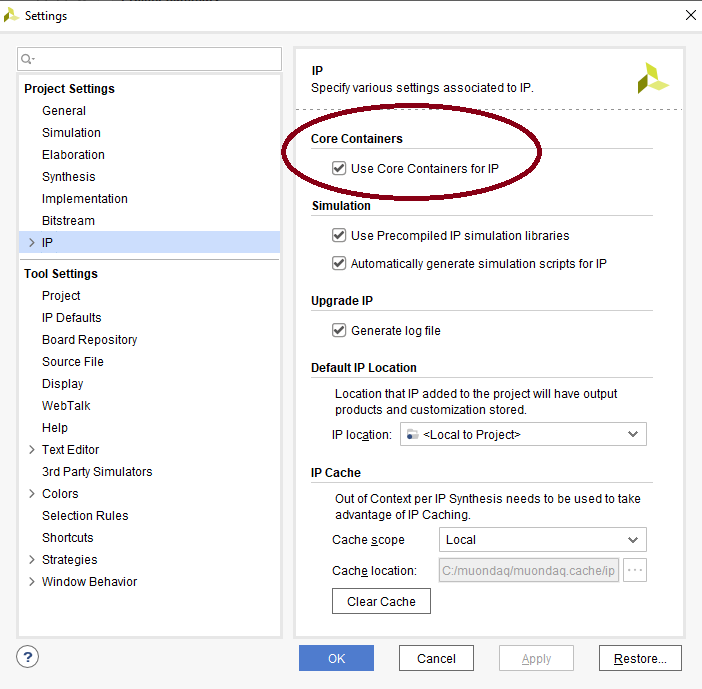
\includegraphics[scale=0.5]{viv1.png}
		\caption{Menú de configuración para la habilitación de IP Containers en Vivado.}
		\label{fig:viv1}
	\end{figure}
	
	Finalmente, se deben importar los archivos contenidos en las carpetas \textit{src, sim, xdc} e \textit{ip} al proyecto de descripción de hardware en la vista \textit{Project Manager} de Vivado.

\section{Exportar script Tcl}

	Desde la interfaz de Vivado se debe exportar el archivo \textit{Tcl} (Tool Command Language) asociado al proyecto Vivado accediendo a \textit{File$>$ Project$>$ Write Tcl} ilustrado en la Figura \ref{fig:viv2} y guardándolo con el nombre \textit{build.tcl} en la carpeta principal de repositorio, no en las subcarpetas creadas. Se debe tener encuentra que el proceso de exportación y edición del archivo Tcl debe realizarse cada vez que se crea o elimina un nuevo archivo fuente del proyecto. En caso de realizar la exportación, el script no generará el proyecto completo y habrá que importar los archivos fuente de manera manual.
	
	\begin{figure}[ht]
		\centering
		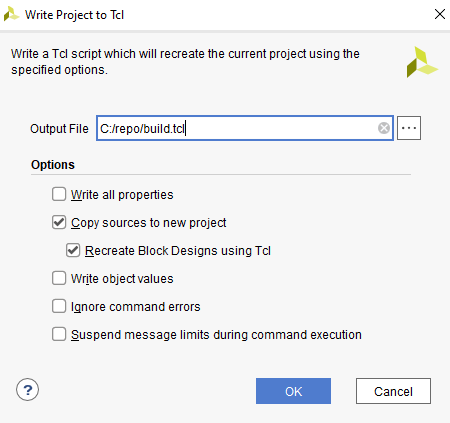
\includegraphics[scale=0.6]{viv2.png}
		\caption{Ventana de Vivado para la exportación de un script Tcl.}
		\label{fig:viv2}
	\end{figure}

\section{Editar script Tcl}
	Un paso importante en este proceso de control de versiones es la edición del archivo Tcl, para que así se generen automáticamente los archivos de Vivado en la carpeta \textit{wd}. Para lograrlo, se debe abrir el archivo \textit{build.tcl} en un editor de texto y buscar los siguientes comandos:

\begin{lstlisting}[language=bash, frame=single, basicstyle=\small]
	
# Set the reference directory for source file relative paths 
#(by default the value is script directory path)
set origin_dir "."

# Set the directory path for the original project from where
#this script was exported
set orig_proj_dir "path-to-the-actual-vivado-project"
	
# Create project
create_project ${_xil_proj_name_} ./${_xil_proj_name_} 
	-part part-of-your-fpga

\end{lstlisting}

	Una vez ubicados, se deben reemplazar por los siguientes comandos:
	
\begin{lstlisting}[language=bash, frame=single, basicstyle=\small]
	
# Set the reference directory for source file relative paths 
#(by default the value is script directory path)
set origin_dir [file dirname [info script]]

# Set the directory path for the original project from where 
#this script was exported
set orig_proj_dir "[file normalize "$origin_dir/wd/"]"

# Create project
create_project ${_xil_proj_name_} $orig_proj_dir/${_xil_proj_name_} 
	-part part-of-your-fpga

\end{lstlisting}


\section{Confirmar y subir los archivos al repositorio remoto}

	En este punto todo se encuentra listo para realizar el primer \textit{commit} en \textit{git} y comenzar el control de versiones del proyecto Vivado mediante el siguiente comando en consola:
	
\begin{lstlisting}[language=bash, frame=single]
$ git add .
$ git commit -m "First commit."
$ git push

\end{lstlisting}

	Luego de ejecutar los comandos en consola, el control de versiones se encuentra correctamente configurado y es seguro eliminar el proyecto Vivado de otras ubicaciones fuera del repositorio, ya que el proyecto puede ser reconstruido completamente al ejecutar el script \textit{ build.tcl} desde la consola Tcl de Vivado.
%
%\chapter{Conexión de señales LVDS en una FPGA Artix 7}
%\label{lvds}
%Este proyecto basa su funcionalidad en un enlace de datos físicos ente una FPGA y una interfaz de lectura ASD, en donde la interfaz emite pulsos digitales através de emisores LVDS internos y FPGA recibe los pulsos mediante un receptor interno. Este apéndice detalla cómo interconectar dispositivos que utilicen interfaces LVDS en cualquier tipo de proyecto, entendiendo los protocolos y requerimientos necesarios para lograrlo.

\section{Acerca del estándar LVDS}	
	LVDS (Low Voltage Differential Signaling) es un enlace de datos de capa física, útiles en aplicaciones que requieran principalmente conservar la integridad de los datos, mantener bajo ruido en el medio de transmisión, o cuando el emisor y receptor se encuentran demasiado lejos el uno del otro.
	
\section{Características principales}
	
	Las interfaces LVDS pueden controlar señales en el rango de los 2V a 5V, con una alta velocidad de transferencia de hasta 500Mbps en un solo par diferencial preservando la integridad de la señal a transmitir y manteniendo una buena inmunidad al ruido y a interferencia por campos electromagnéticos Se caracterizan por ser económicas, de bajo consumo de potencia, pequeñas y de una implementación simple.

	Las interfaces LVDS transfieren datos a través de una linea de par trenzado en la que los voltajes de cada alambre tienen opuesta amplitud de voltaje. Estas señales son montadas sobre un nivel de voltaje continuo típicamente de 1,2V y poseen tan solo 400mV de diferencia de voltaje ente ambos alambres. La Figura IMAGE ilustra estos niveles de voltaje.
	
	La Figura IMAGE ilustra las señales LVDS, mostrando primero una señal de una linea para luego ilustrar la señal diferencial en sí misma. V$_{idth}$ (Input Differential Threshold Voltage) corresponde al nivel de voltaje después de que el receptor capura la señal diferencial entrante.  V$_{ob}$ corresponde al alambre con potencial de voltaje positivo,  V$_{oa}$ corresponde al alambre de potencial negativo y  V$_{od}$ representa la diferencia de voltaje final ente el par de alambres.
	
	Los las interfaces diferenciales solamente emiten y reciben la diferencia entre los dos alambre que componen la linea de transmisión, eliminando el ruido de modo común en la señal de voltaje asociado a la diferencia de voltaje existente entre la tierra eléctrica , el emisor y el receptor, sumado al ruido propio infiltrado en la linea de transmisión.
	
	La implementación de una linea de datos LVDS requiere un emisor, una linea de transmisión, un resistor de 100$\Omega$ y un receptor, como se observa en la Figura IMAGE. El resistor de 100$\Omega$ se debe a la impedancia propia de la linea de transmisión (50$\Omega$) de cada alambre respecto a tierra, junto a una linea de transmisión simétrica se obtiene un medio de comunicación que mantiene la adaptación de impedancia y la integridad de la señal enviada. 


\section{Interconexión LVDS para hardware Xilinx Series 7}

	La familia de FPGAS Xilinx 7 series son capaces de operar con señales LVDS tanto en su emisión como recepción, con la opción de habilitar un resistor de 100$\Omega$ en caso de que el circuito conectado no cuente con él. Además, esta familia de FPGAS cuenta con dos tipos de estándar LVDS, el LVDS común que requiere una fuente de 1.8V y se encuentra disponible en los bancos HP (High Performance) de la FPGA, y el están LVDS\_25, el cual necesita una fuente de voltaje de 2,5V para alimentar sus bancos de puertos correspondientes unicamente a los de tipo HR (High Rank). Usar cualquiera de estos dos estándares con su correcta fuente de voltaje permita habilitar o deshabilitar el resistor interno, de lo contrario, en el caso de usar un voltaje diferente se debe mantener el resistor interno desactivado.
	
	En particular, la FPGA Artix 7 y la Zynq 7000 tienen solamente bancos HR, por lo que solo está disponible el estándar LVDS\_25, pero las tarjetas Trenz utilizadas en esta memoria de titulación solo cuentan con fuentes de 1,8V, 3,3V y 5V, lo que implica que para utilizar el resistor interno se debe utilizar una fuente de voltaje externa de 2,5V

\section{Descripción de hardware para utilización de puertos LVDS}

	Para operar correctamente utilizando puertos LVDS en la familia de FPGAs Xilinx 7 series es necesario declarar los puertos a utilizar y el voltaje asociado en el archivo de \textit{constraints} XDC. Por ejemplo para utilizar el par diferencial B16\_L22\_P (positivo) y B16\_L22\_N (negativo) ubicados respectivamente en los puertos E22 y D22 de la FPGA, se declararían las siguientes lineas:
	
	CODIGO

%set_property -dict {PACKAGE_PIN E22 IOSTANDARD LVDS_25} [get_ports B16_L22_P];
%set_property -dict {PACKAGE_PIN D22 IOSTANDARD LVDS_25} [get_ports B16_L22_N];

	Finalmente, para poder utilizar correctamente el par diferencial, es necesario utilizar un \textit{IO Buffer} instanciado en el hardware descrito. Estos buffers permiten convertir la señal diferencial a una de un solo terminal o viceversa. Por ejemplo, para usar un par diferencial según el estándar LVDS\_25 habilitando la resistencia interna del puerto, bastaria con declarar un IBUFDS (Input Buffer for Differential Singal) como se indica a continuación:
	
	CODIGO:


%// IBUFDS: Differential Input Buffer - Verilog
%// 7 Series
%// Xilinx HDL Libraries Guide, version 13.4
%IBUFDS #(
%    .DIFF_TERM("TRUE"), // Differential Termination (TRUE or FALSE)
%    .IBUF_LOW_PWR("FALSE"), // Low power="TRUE", Highest performance="FALSE"
%    .IOSTANDARD("LVDS_25") // Specify the input I/O standard (LVDS or LVDS_25)
%    ) IBUFDS_LVDS_25 (
%    .O(lvds_output), // Buffer output
%    .I(B16_L22_P), // Diff_p buffer input (connect directly to top-level port)
%    .IB(B16_L22_N) // Diff_n buffer input (connect directly to top-level port)
%);
%// End of IBUFDS_inst instantiation

Siguiendo estos pasos, el receptor LVDS queda correctamente configurado. Para utilizar el receptor basta con conectar las respectivas señales diferenciales en los puertos correspondientes declarados en el diseño y utilizar un cable de par trenzado simétrico con una impedencia de 50$\Omega$.
%
%\chapter{Ajuste de forma en pulsos electrónicos para la física}
%\label{shaping}
% 
%
%\chapter{Rayos cósmicos y partículas de alta energía}
%\label{muon}
%\input{Appx_muon.tex}

%%
%%%%------------------BIBLIOGRAFÍA-----------------------------
%%%

\bibliographystyle{IEEEtran}
\bibliography{references}

\end{document}







